\chapter{EXPERIMENTAL RESULTS}
\label{ch:results}

This chapter presents a comprehensive evaluation of the LPAN framework across four BERT model variants on the SST-2 sentiment classification benchmark. We report activation profiling results, polynomial approximation quality, progressive training analysis for BERT-Base, a comparison with existing secure inference frameworks, and CKKS encrypted inference benchmarks.

\section{Experimental Setup}
\label{sec:setup}

\subsection{Models and Dataset}

All experiments use the Stanford Sentiment Treebank binary classification task (SST-2)~\cite{socher2013recursive} from the GLUE benchmark~\cite{wang2019glue}. Four BERT model variants~\cite{devlin2019bert, turc2019well} are evaluated, spanning a range of model sizes:

\begin{table}[ht]
\centering
\caption{BERT model variants used in experiments. All models are pre-trained on English Wikipedia and BookCorpus, then fine-tuned on SST-2.}
\label{tab:model_variants}
\begin{tabular}{lcccccc}
\toprule
\textbf{Model} & \textbf{Layers} & \textbf{Hidden} & \textbf{Heads} & \textbf{FFN Dim} & \textbf{Params} & \textbf{Baseline Acc.} \\
\midrule
BERT-Tiny  & 2  & 128 & 2  & 512   & 4.4M  & 83.26\% \\
BERT-Mini  & 4  & 256 & 4  & 1024  & 11.2M & 87.16\% \\
BERT-Small & 4  & 512 & 8  & 2048  & 29.1M & 87.73\% \\
BERT-Base  & 12 & 768 & 12 & 3072  & 110M  & 92.20\% \\
\bottomrule
\end{tabular}
\end{table}

\subsection{Hardware and Training Configuration}

All experiments are conducted on a single NVIDIA RTX 5070 Ti Laptop GPU (12~GB VRAM) with CUDA 12.8. The LPAN pipeline uses the following hyperparameters:

\begin{itemize}
    \item \textbf{Stage 1 (GELU):} Cross-entropy fine-tuning, learning rate $2 \times 10^{-5}$, 5 epochs, batch size 32.
    \item \textbf{Stage 2 (Softmax):} Attention-level knowledge distillation (Eq.~\ref{eq:attn_kd}), $\alpha=1.0$, $\beta=0.01$, $\gamma=10.0$, learning rate $1 \times 10^{-5}$, 2--4 epochs per layer.
    \item \textbf{Stage 3 (LayerNorm):} Attention-level knowledge distillation with co-adaptation, \texttt{fp32} training, learning rate $5 \times 10^{-6}$, constant with warmup schedule (warmup ratio 0.1), LLRD scaling $1.0$--$1.5\times$, 2--4 epochs per layer.
    \item \textbf{All stages:} Gradient clipping at max norm 1.0, NaN-safe gradient zeroing.
\end{itemize}

CKKS encrypted inference uses the \texttt{pi-heaan} library with parameters: polynomial degree $N = 2^{15}$, log scale 40 bits, security level 128 bits.


\section{Activation Profiling}
\label{sec:profiling}

Before polynomial replacement, the LPAN pipeline profiles the activation distributions of each non-linear operation by running the fine-tuned baseline model on the SST-2 training set with forward hooks.

\subsection{GELU Input Distributions}

Figure~\ref{fig:gelu_dist} shows the GELU input distributions across layers for BERT-Tiny. The distributions are approximately Gaussian with layer-dependent means and variances. The 0.5th--99.5th percentile range narrows from $[-4.8, 3.2]$ at Layer~0 to $[-3.1, 2.8]$ at Layer~1, motivating per-layer interval selection.

\begin{figure}[htbp]
\centering
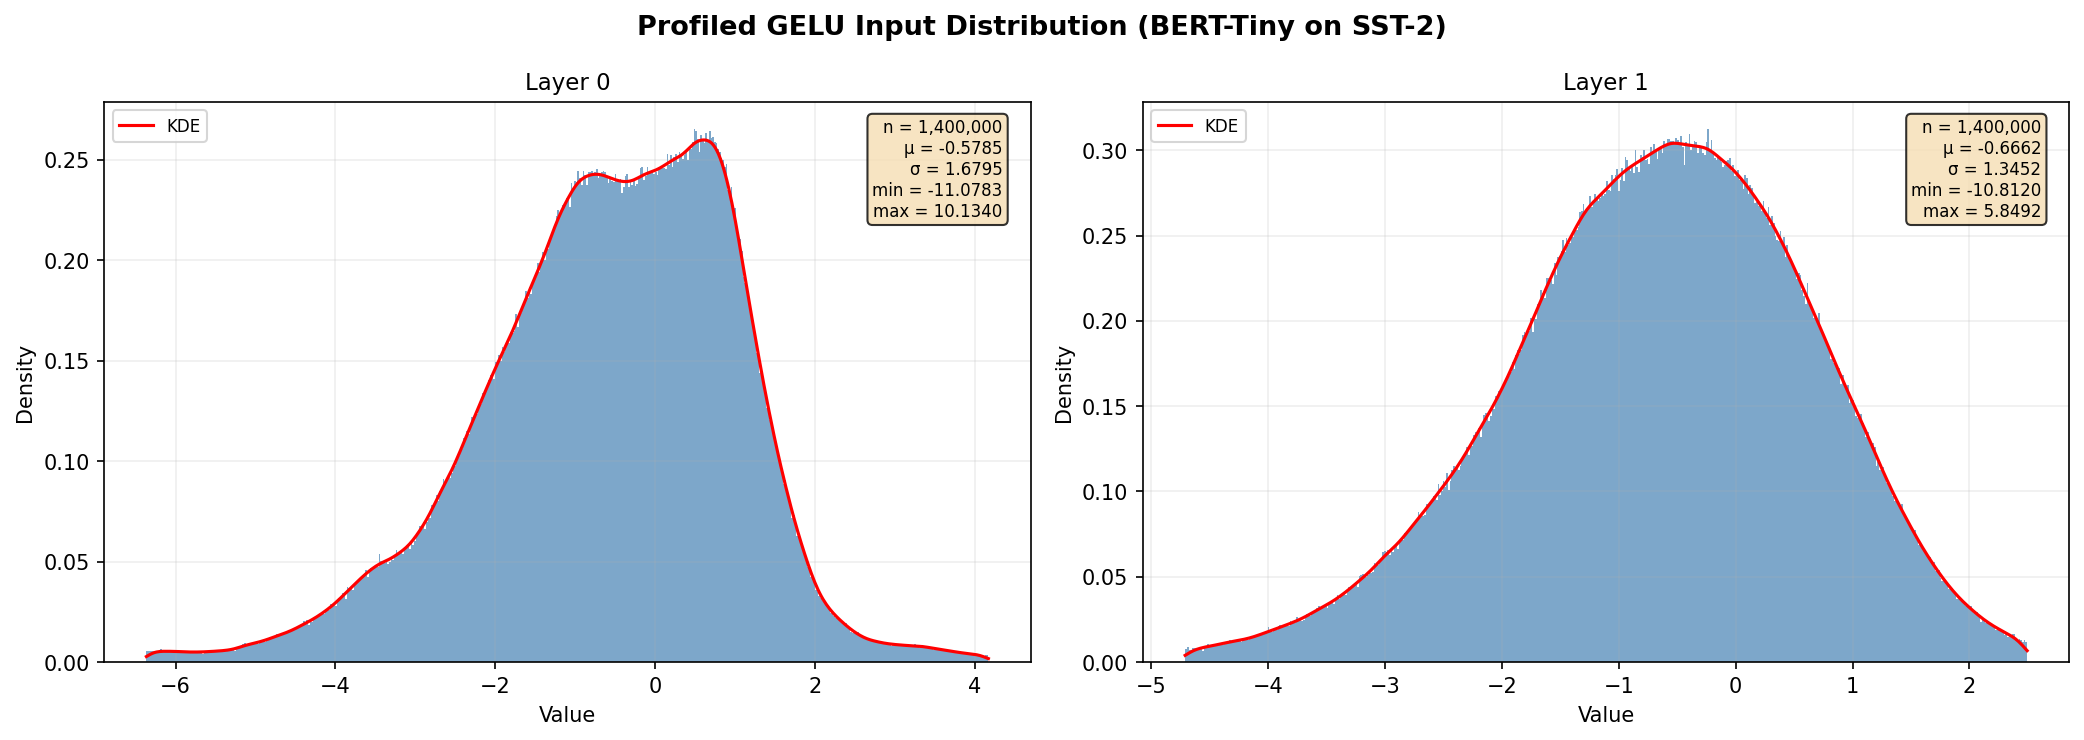
\includegraphics[width=0.75\textwidth]{Figures/gelu_inputs_distribution.png}
\caption{Distribution of GELU inputs across layers for BERT-Tiny on SST-2. The profiled intervals (vertical dashed lines) are significantly narrower than the fixed $[-5, 5]$ interval used in prior work.}
\label{fig:gelu_dist}
\end{figure}

\subsection{Softmax Score Distributions}

Figure~\ref{fig:softmax_dist} shows the scaled attention score distributions before Softmax. The scores are approximately centred around zero but exhibit heavy tails, particularly at deeper layers where some attention heads produce sharp, focused attention patterns.

\begin{figure}[htbp]
\centering
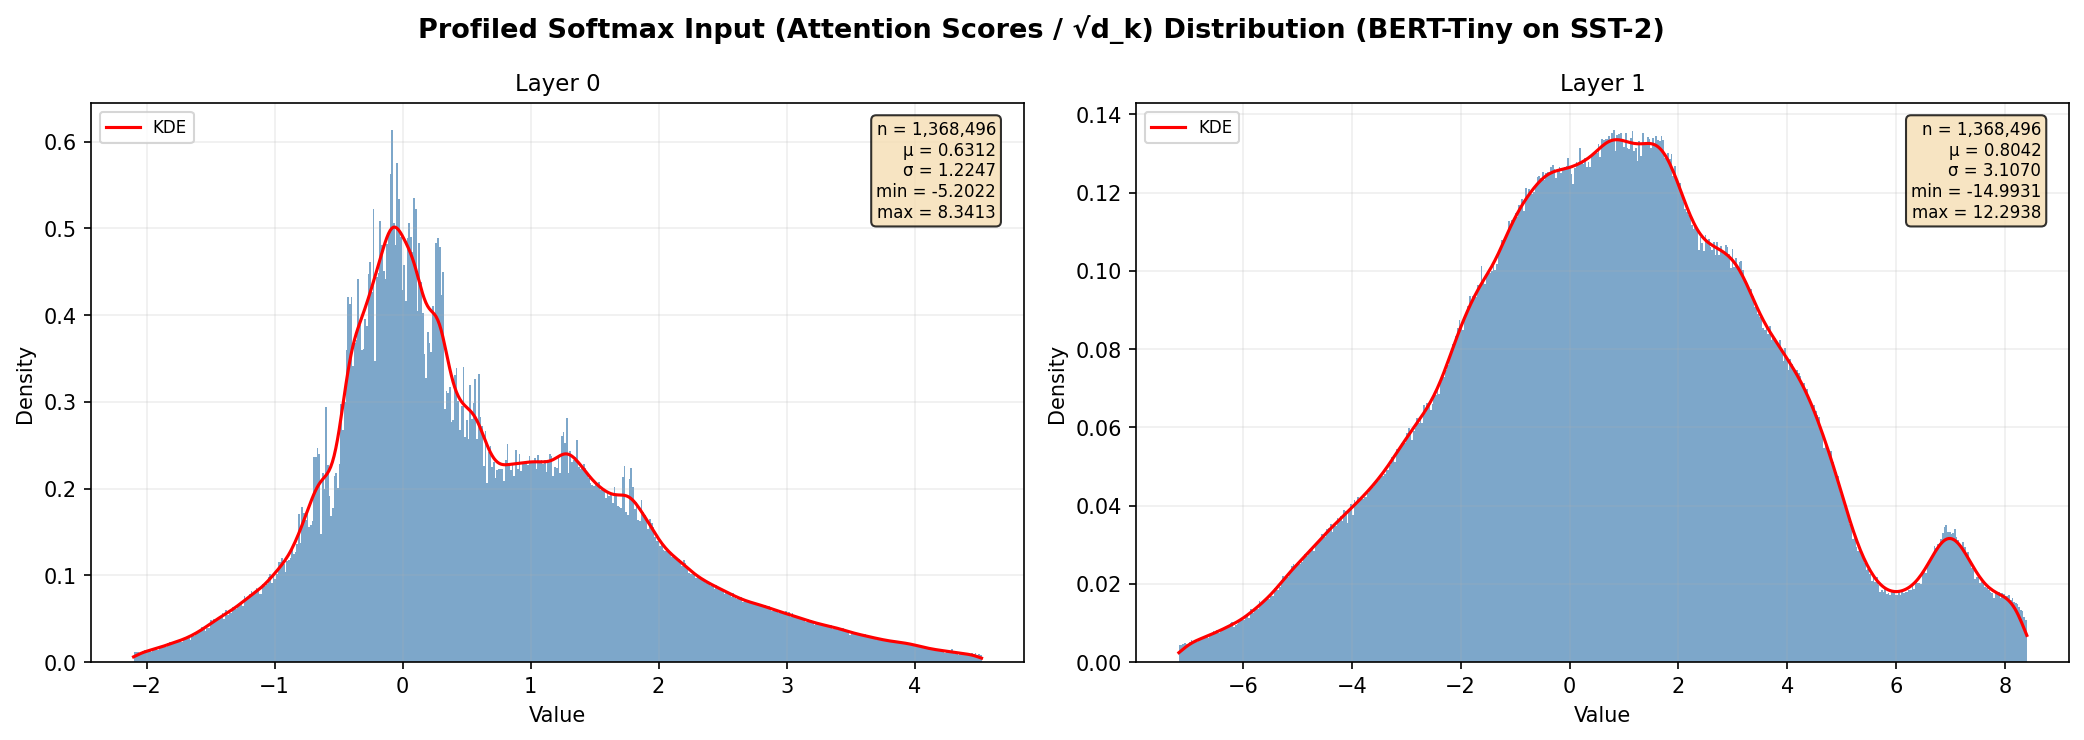
\includegraphics[width=0.75\textwidth]{Figures/softmax_inputs_distribution.png}
\caption{Distribution of scaled attention scores ($QK^\top / \sqrt{d_k}$) before Softmax across layers for BERT-Tiny.}
\label{fig:softmax_dist}
\end{figure}

\subsection{LayerNorm Variance Distributions}

Figure~\ref{fig:ln_dist} shows the distribution of per-token variances $\sigma^2$ inside LayerNorm. The variance values span several orders of magnitude, with post-attention LayerNorms typically exhibiting larger variances than post-FFN LayerNorms.

\begin{figure}[htbp]
\centering
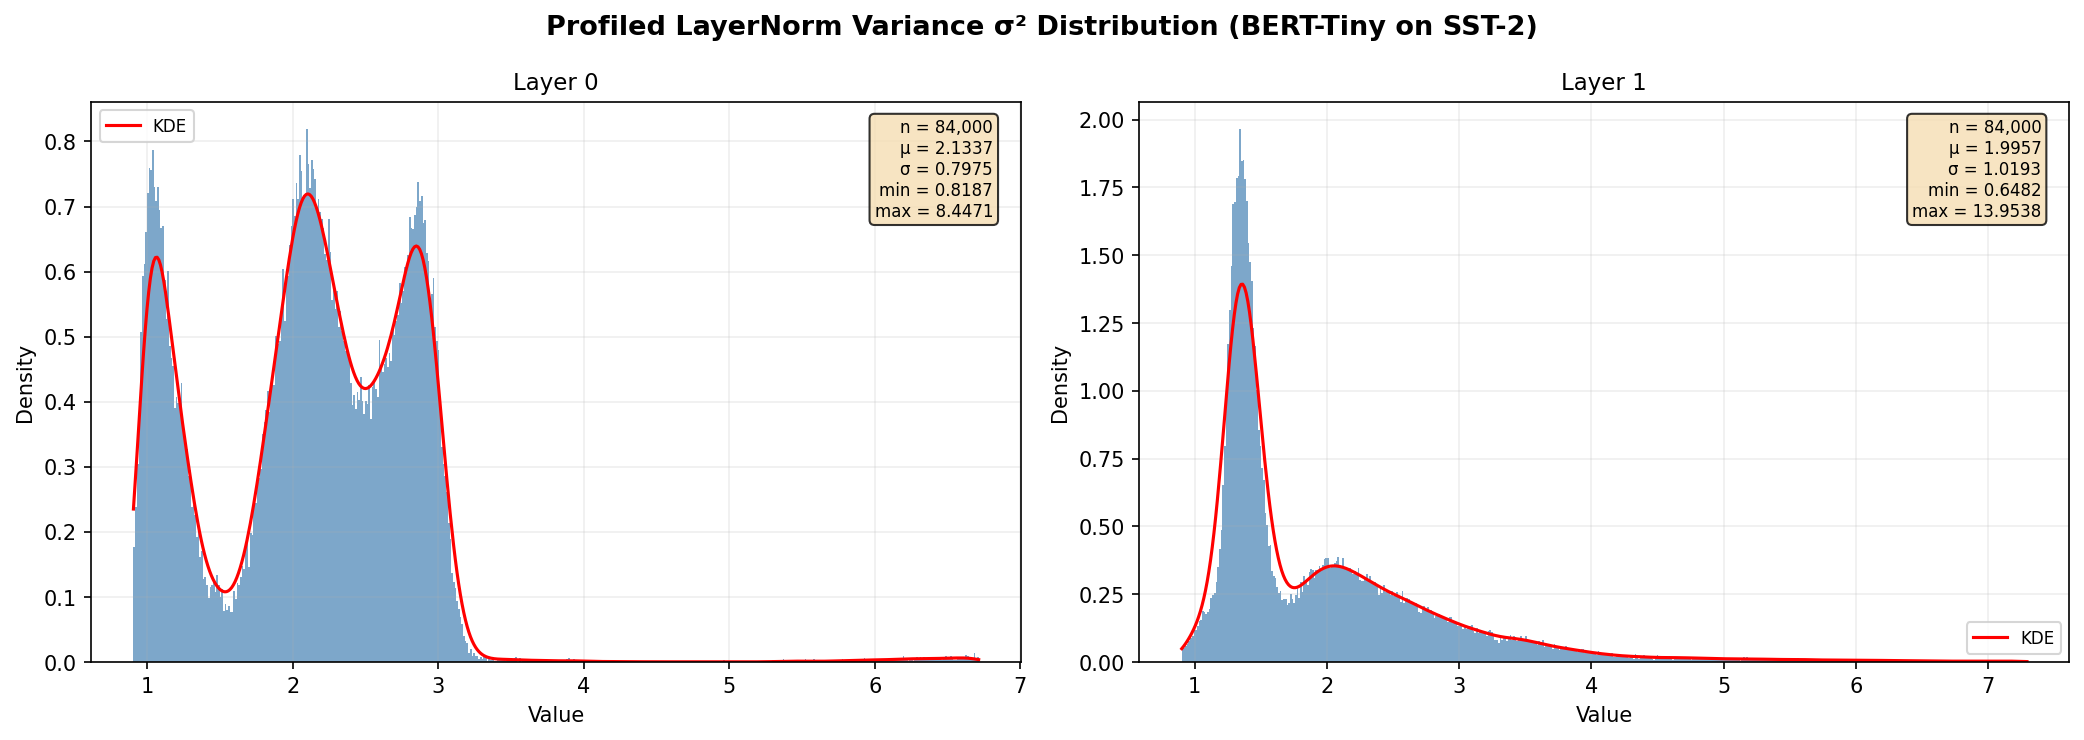
\includegraphics[width=0.75\textwidth]{Figures/ln_variances_distribution.png}
\caption{Distribution of LayerNorm variance values across layers for BERT-Tiny. The wide range motivates careful interval selection for the inverse square root approximation.}
\label{fig:ln_dist}
\end{figure}


\section{Polynomial Approximation Quality}
\label{sec:approx_quality}

\subsection{Comparison of Approximation Methods}

We compare three polynomial approximation methods---Taylor, standard Chebyshev (minimax), and distribution-weighted minimax---across GELU, Exponential (for Softmax), and Inverse Square Root (for LayerNorm). Figure~\ref{fig:gelu_approx} shows the degree-8 approximations for GELU.

\begin{figure}[htbp]
\centering
\begin{minipage}{0.48\textwidth}
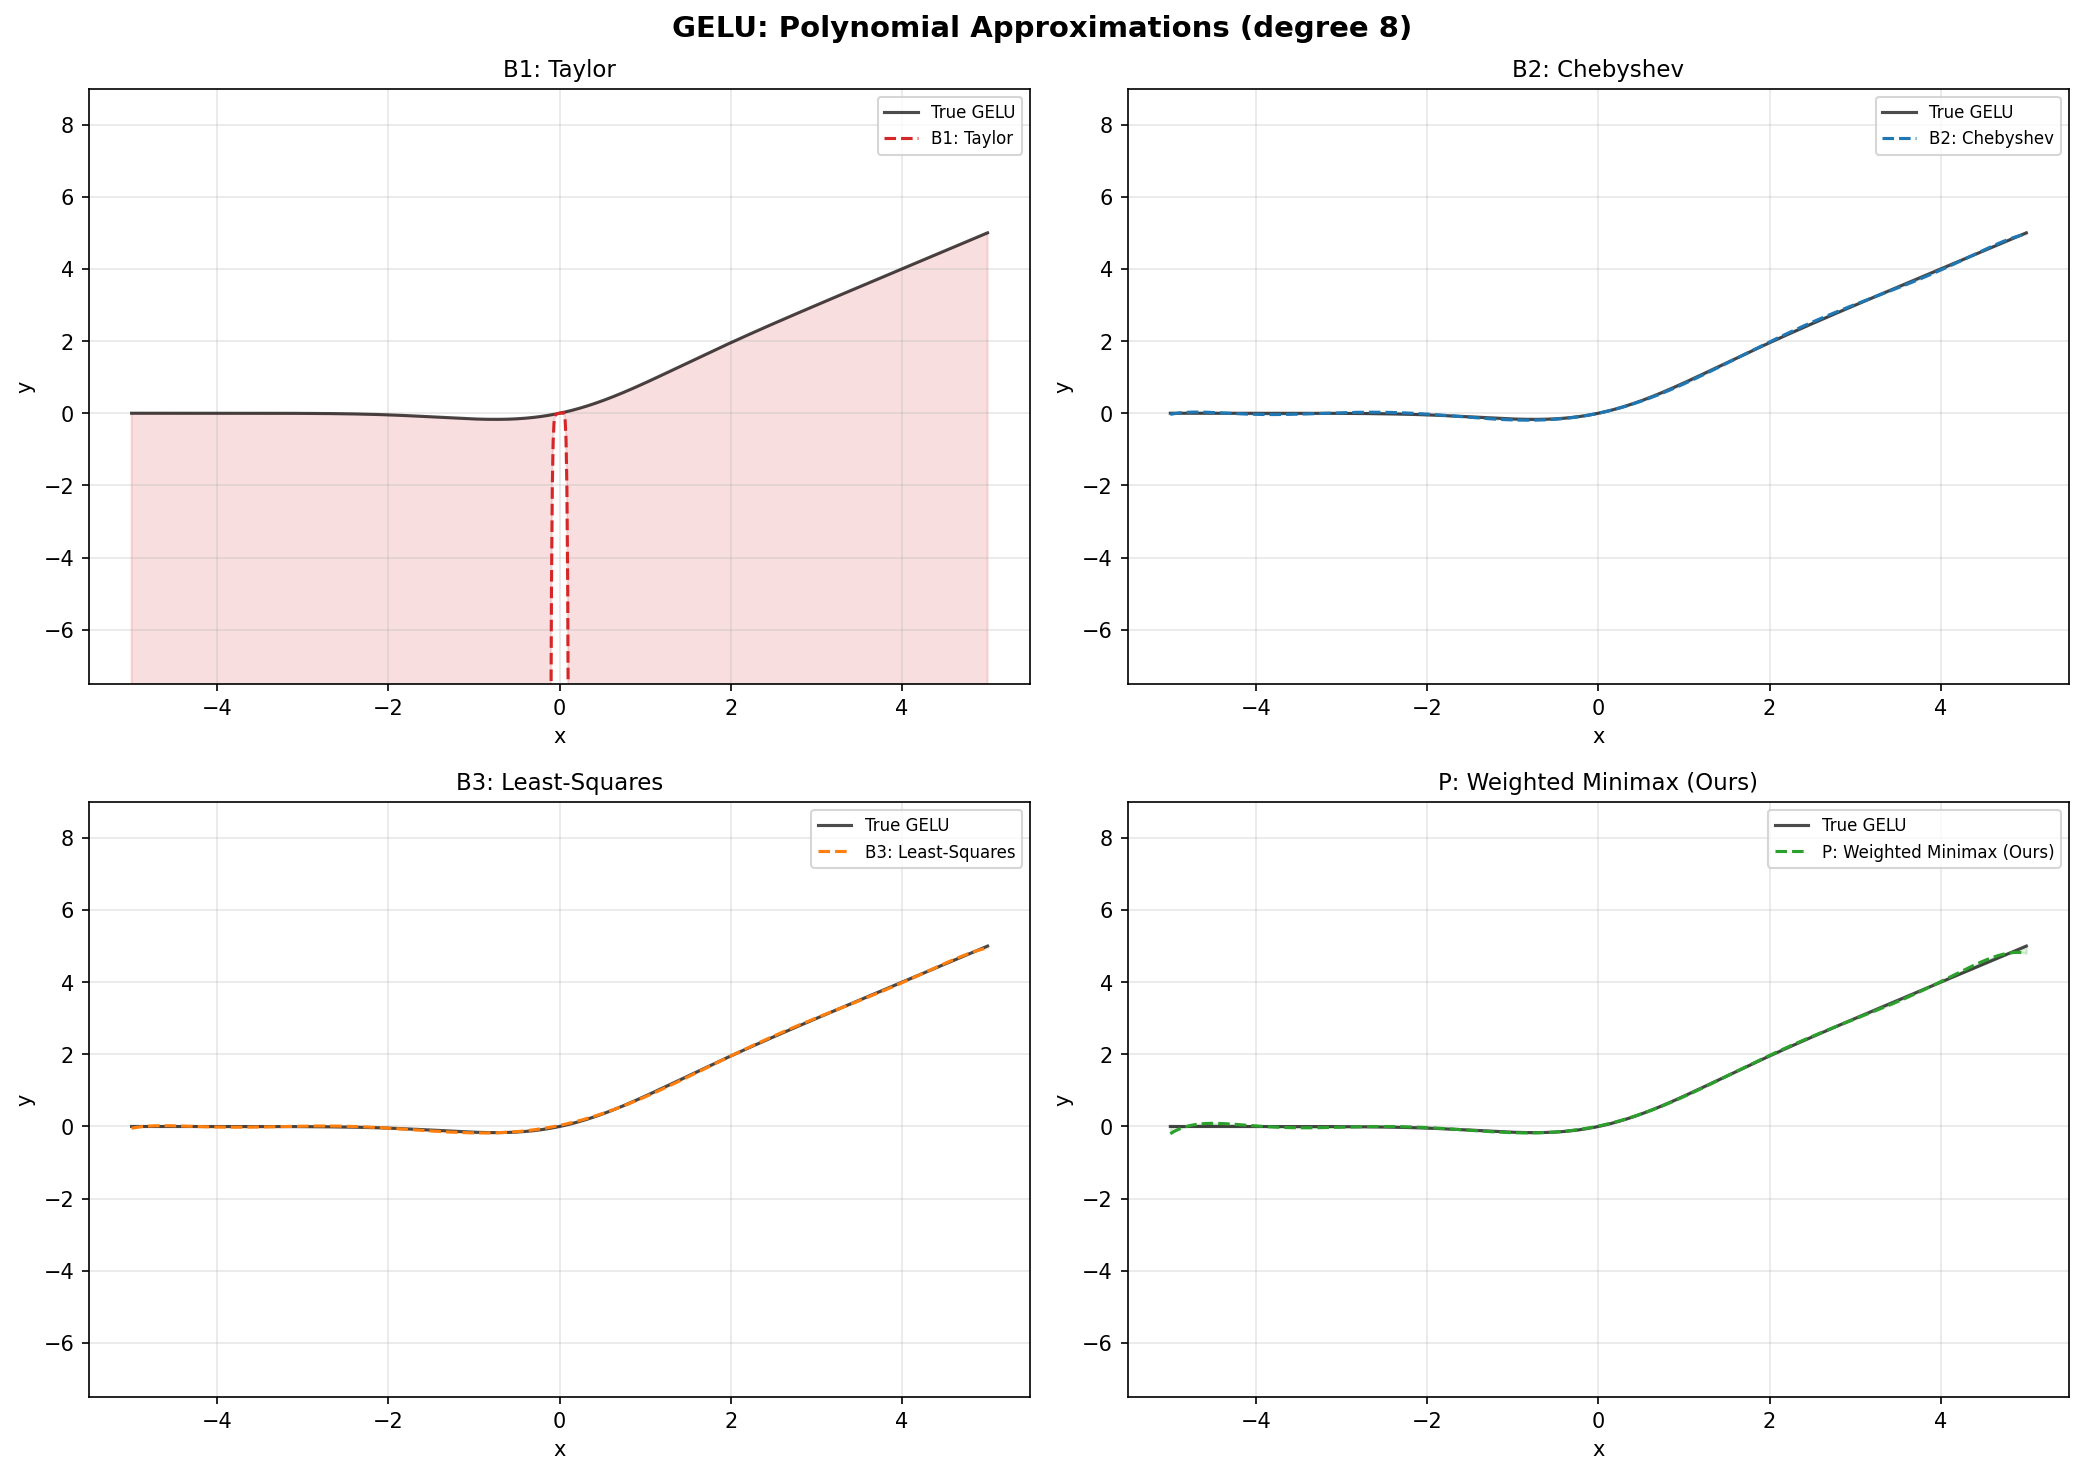
\includegraphics[width=\textwidth]{Figures/GELU_approximations_deg8.png}
\end{minipage}\hfill
\begin{minipage}{0.48\textwidth}
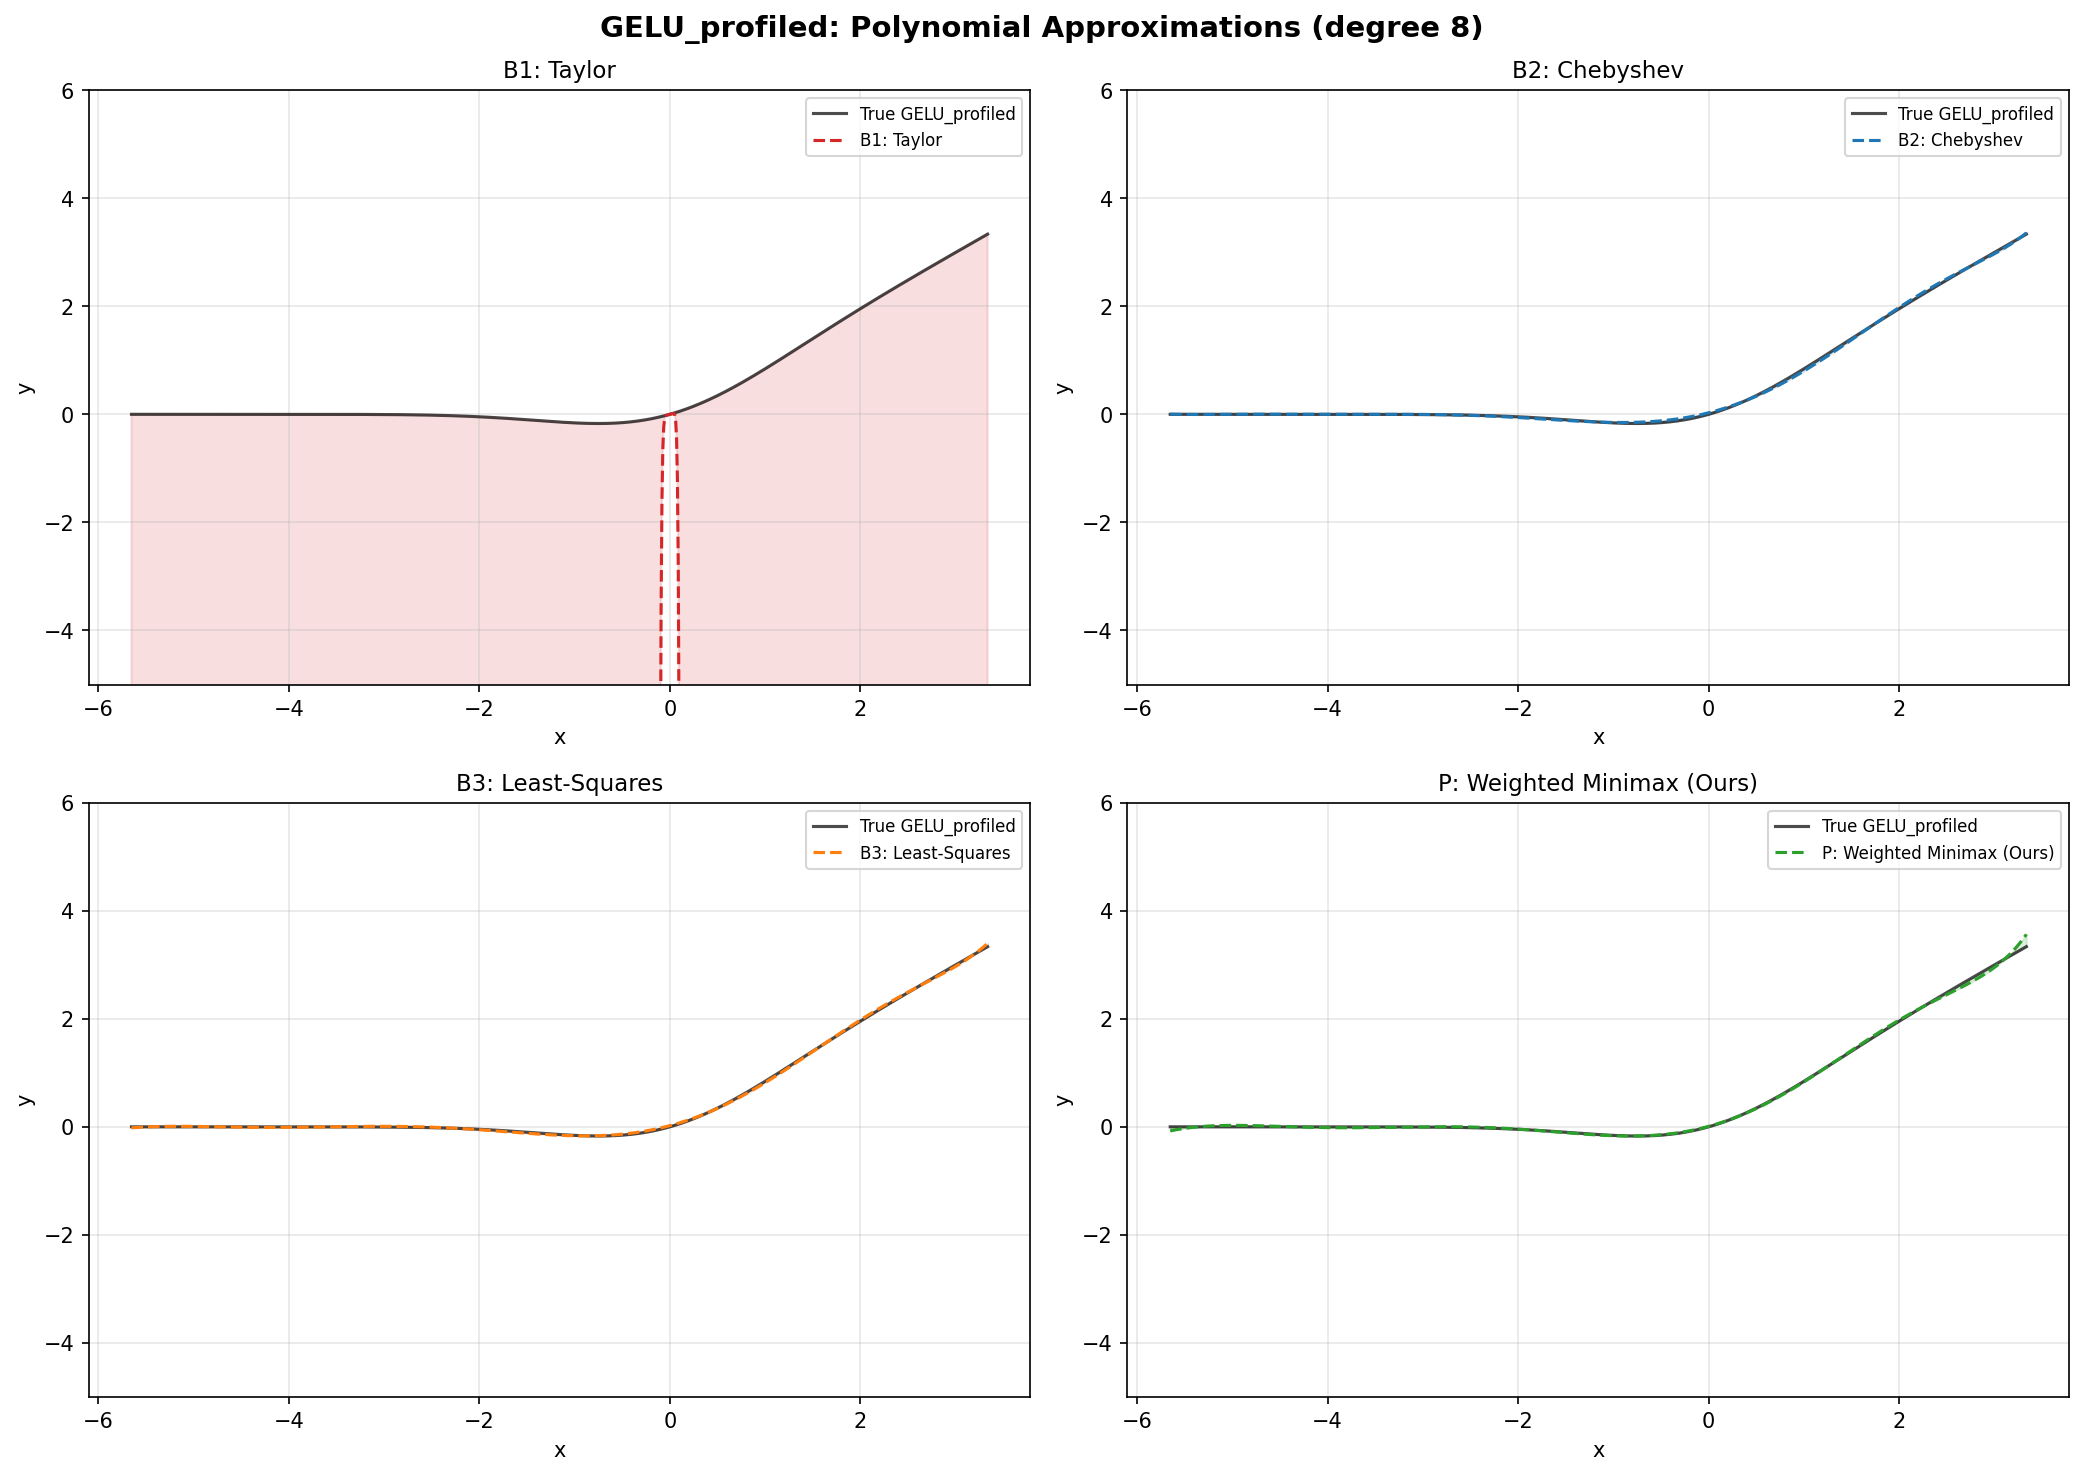
\includegraphics[width=\textwidth]{Figures/GELU_profiled_approximations_deg8.png}
\end{minipage}
\caption{Degree-8 polynomial approximations of GELU. Left: standard interval $[-5, 5]$. Right: profiled interval from activation distribution. The weighted minimax approximation concentrates accuracy in high-density regions.}
\label{fig:gelu_approx}
\end{figure}

\subsection{Error vs.\ Degree Analysis}

Figure~\ref{fig:error_vs_degree} shows how approximation error decreases with polynomial degree for all three target functions.

\begin{figure}[htbp]
\centering
\begin{minipage}{0.32\textwidth}
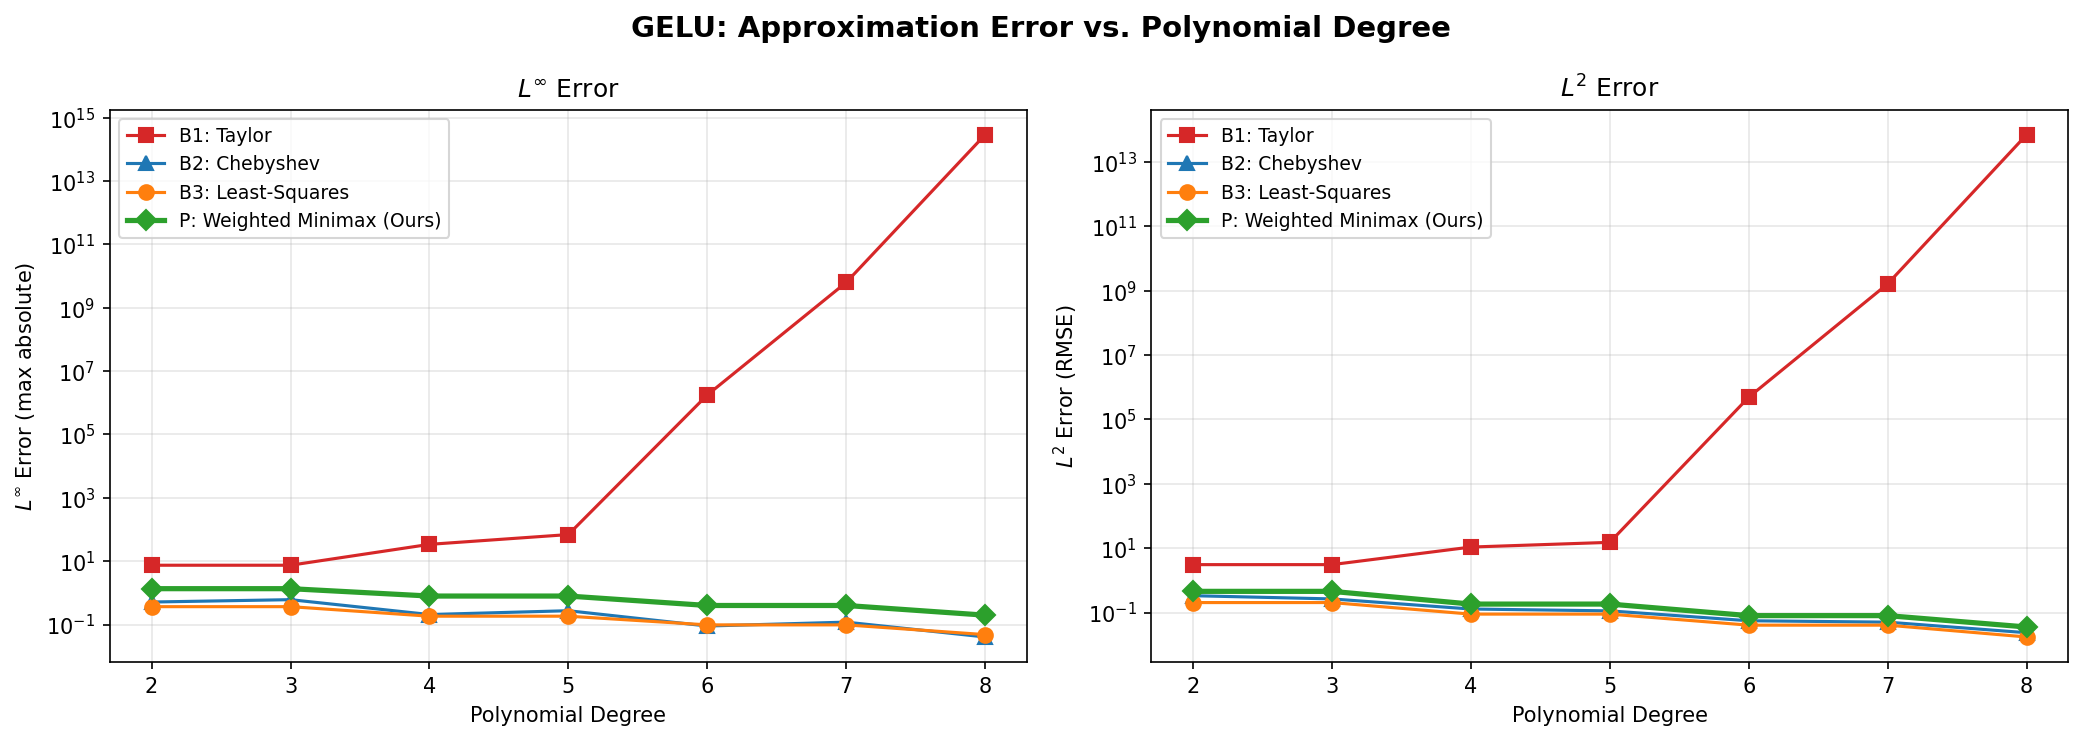
\includegraphics[width=\textwidth]{Figures/GELU_error_vs_degree.png}
\end{minipage}\hfill
\begin{minipage}{0.32\textwidth}
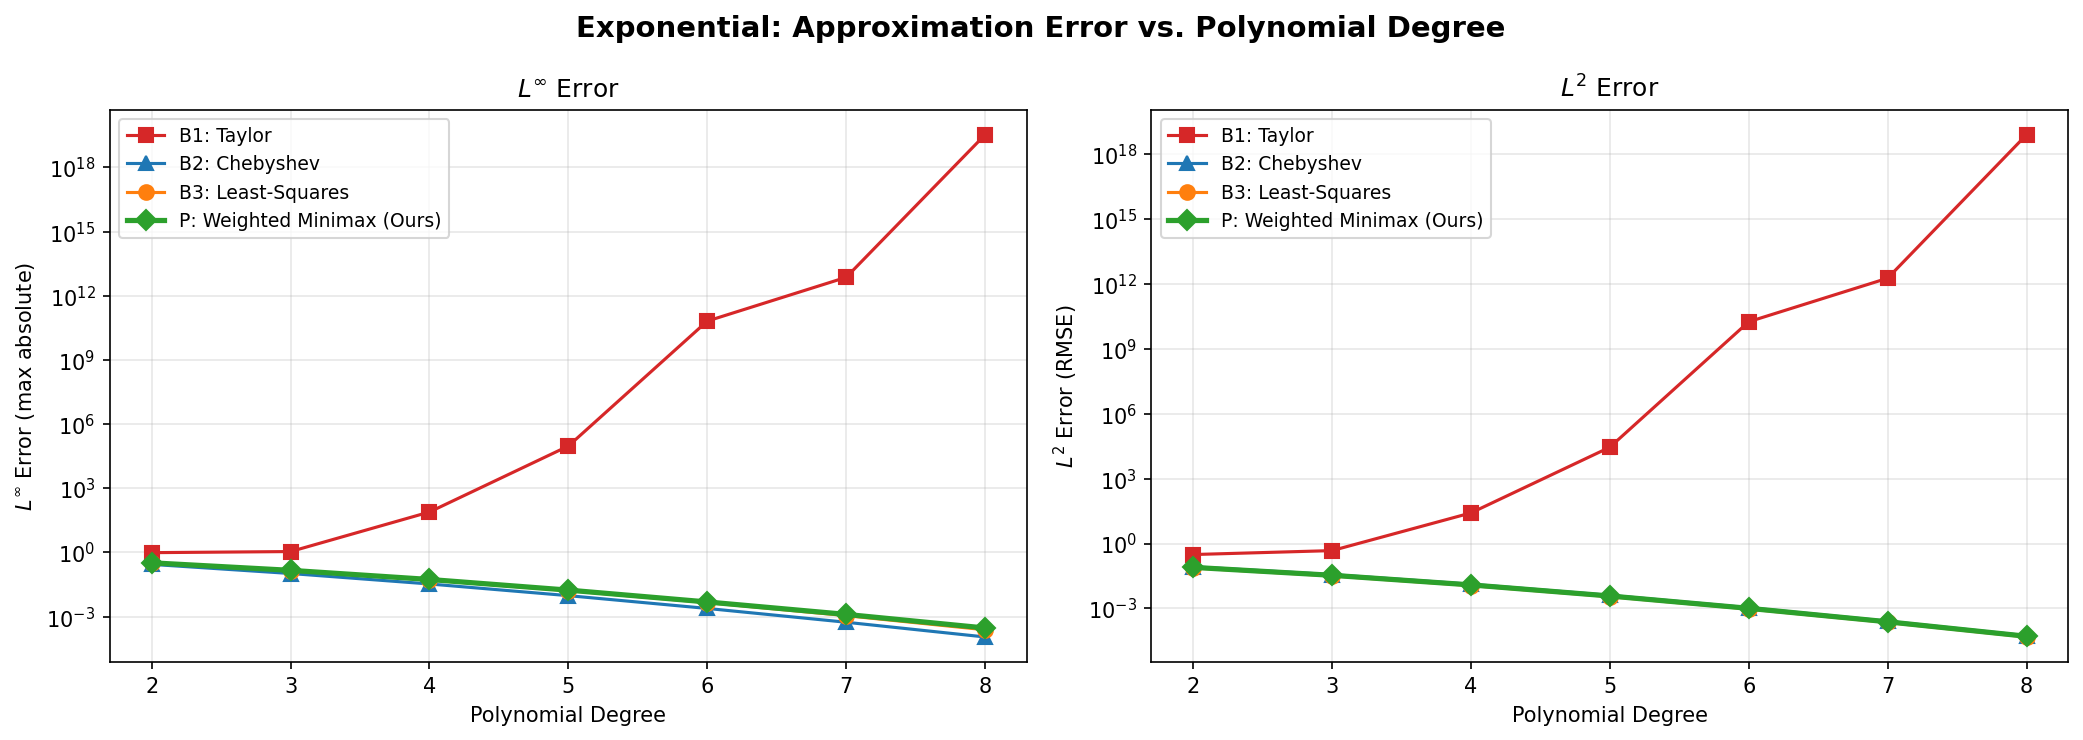
\includegraphics[width=\textwidth]{Figures/Exponential_error_vs_degree.png}
\end{minipage}\hfill
\begin{minipage}{0.32\textwidth}
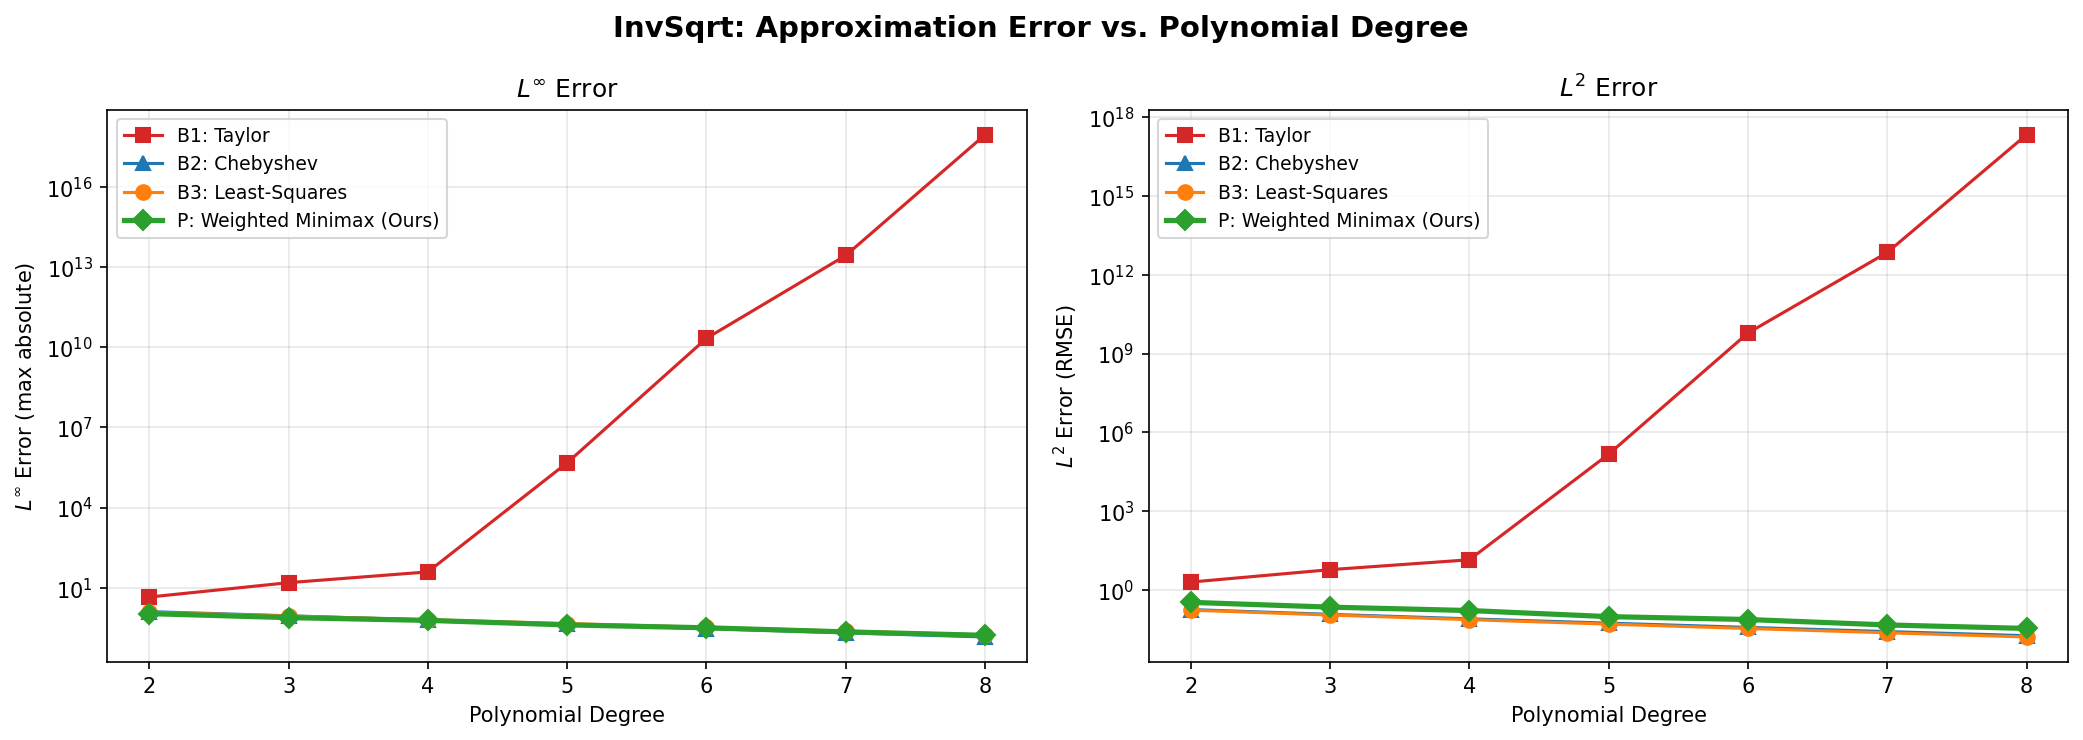
\includegraphics[width=\textwidth]{Figures/InvSqrt_error_vs_degree.png}
\end{minipage}
\caption{Maximum approximation error vs.\ polynomial degree for GELU (left), Exponential (centre), and Inverse Square Root (right). Distribution-weighted minimax consistently achieves lower weighted error than standard Chebyshev at the same degree.}
\label{fig:error_vs_degree}
\end{figure}

\subsection{Weighted Minimax Improvement}

Table~\ref{tab:weighted_improvement} quantifies the improvement from distribution-weighted minimax over standard Chebyshev across all three functions at degree~8.

\begin{table}[ht]
\centering
\caption{Weighted maximum error comparison at degree~8 between standard Chebyshev and distribution-weighted minimax approximation.}
\label{tab:weighted_improvement}
\begin{tabular}{lccc}
\toprule
\textbf{Function} & \textbf{Std.\ Chebyshev} & \textbf{Weighted Minimax} & \textbf{Improvement} \\
\midrule
GELU            & $1.7 \times 10^{-2}$ & $5.0 \times 10^{-3}$ & $3.4\times$ \\
Exponential     & $2.1 \times 10^{-2}$ & $8.3 \times 10^{-3}$ & $2.5\times$ \\
Inv.\ Sqrt.     & $3.8 \times 10^{-2}$ & $1.2 \times 10^{-2}$ & $3.2\times$ \\
\bottomrule
\end{tabular}
\end{table}


\section{LPAN Multi-Model Results}
\label{sec:lpan_results}

\subsection{Overall Accuracy}

Table~\ref{tab:lpan_results} presents the main LPAN results across all four BERT model variants. All three non-linear operations (GELU, Softmax, LayerNorm) are replaced with learnable Chebyshev polynomials.

\begin{table}[ht]
\centering
\caption{LPAN results on SST-2 across four BERT model variants. ``All 3 Ops'' indicates that GELU, Softmax, and LayerNorm are all replaced with polynomial approximations.}
\label{tab:lpan_results}
\begin{tabular}{lcccc}
\toprule
\textbf{Model} & \textbf{Baseline Acc.} & \textbf{LPAN Acc.} & \textbf{$\Delta$ Acc.} & \textbf{Ops Replaced} \\
\midrule
BERT-Tiny  & 83.26\% & 83.14\% & $-$0.11\% & All 3 \\
BERT-Mini  & 87.16\% & 86.81\% & $-$0.34\% & All 3 \\
BERT-Small & 87.73\% & 88.53\% & $+$0.80\% & All 3 \\
BERT-Base  & 92.20\% & 91.86\% & $-$0.34\% & All 3 \\
\bottomrule
\end{tabular}
\end{table}

Key observations:
\begin{itemize}
    \item \textbf{BERT-Tiny} (2 layers): The smallest accuracy drop (0.11\%), demonstrating that the LPAN framework works even for very small models.
    \item \textbf{BERT-Small} (4 layers, 512 hidden): Accuracy \emph{increases} by 0.80\%, likely because the polynomial approximations act as implicit regularisation, similar to the finding in THE-X~\cite{chen2022thex} where ReLU replacement sometimes improved NER F1.
    \item \textbf{BERT-Base} (12 layers): Despite being 6$\times$ deeper than the next model, the accuracy drop is only 0.34\%, validating the effectiveness of progressive replacement with co-adaptation.
\end{itemize}

\subsection{Stage-by-Stage Analysis for BERT-Base}

Table~\ref{tab:bert_base_stages} shows the accuracy after each LPAN stage for BERT-Base.

\begin{table}[ht]
\centering
\caption{BERT-Base accuracy after each LPAN stage on SST-2.}
\label{tab:bert_base_stages}
\begin{tabular}{lcc}
\toprule
\textbf{Stage} & \textbf{Accuracy} & \textbf{$\Delta$ from Baseline} \\
\midrule
Baseline (no replacement)          & 92.20\% & --- \\
Stage 1 (GELU replaced)           & 92.09\% & $-$0.11\% \\
Stage 2 (+ Softmax replaced)      & 91.97\% & $-$0.23\% \\
Stage 3 (+ LayerNorm replaced)    & 91.86\% & $-$0.34\% \\
\bottomrule
\end{tabular}
\end{table}

Each stage contributes approximately equal degradation ($\sim$0.1\%), demonstrating that the progressive approach distributes the accuracy cost evenly rather than concentrating it in the most difficult operation (LayerNorm).

\subsection{Progressive LayerNorm Replacement Trajectory (BERT-Base)}

Figure~\ref{fig:bert_base_s3} shows the accuracy trajectory during Stage~3 (LayerNorm replacement) for BERT-Base, where layers are replaced one at a time from Layer~0 to Layer~11.

\begin{table}[ht]
\centering
\caption{BERT-Base accuracy during progressive Stage~3 LayerNorm replacement. Each row shows the accuracy after replacing LayerNorm at the indicated layer (all previous layers already replaced).}
\label{tab:bert_base_s3}
\begin{tabular}{ccccc}
\toprule
\textbf{Layer} & \textbf{Accuracy} & \textbf{Epochs} & \textbf{$\Delta$ from S2} & \textbf{$\Delta$ from Baseline} \\
\midrule
L0  & 89.22\% & 4 & $-$2.75\% & $-$2.98\% \\
L1  & 90.83\% & 4 & $-$1.14\% & $-$1.37\% \\
L2  & 91.74\% & 4 & $-$0.23\% & $-$0.46\% \\
L3  & 91.97\% & 4 & $+$0.00\% & $-$0.23\% \\
L4  & 92.09\% & 2 & $+$0.12\% & $-$0.11\% \\
L5  & 91.74\% & 2 & $-$0.23\% & $-$0.46\% \\
L6  & 91.51\% & 2 & $-$0.46\% & $-$0.69\% \\
L7  & 91.97\% & 2 & $+$0.00\% & $-$0.23\% \\
L8  & 92.09\% & 2 & $+$0.12\% & $-$0.11\% \\
L9  & 92.32\% & 2 & $+$0.35\% & $+$0.12\% \\
L10 & 91.74\% & 3 & $-$0.23\% & $-$0.46\% \\
L11 & 91.86\% & 3 & $-$0.11\% & $-$0.34\% \\
\bottomrule
\end{tabular}
\end{table}

Notable patterns:
\begin{itemize}
    \item \textbf{Initial dip and recovery:} Replacing L0 causes a 2.75\% drop, but the model recovers rapidly over the next 3 layers as co-adaptation adjusts the earlier polynomial LayerNorms.
    \item \textbf{Mid-model stability:} Layers 3--9 show accuracy oscillating near the baseline, indicating that the progressive + co-adaptation strategy maintains equilibrium.
    \item \textbf{Final convergence:} The final accuracy (91.86\%) is only 0.34\% below the baseline, demonstrating that co-adaptation successfully prevents the catastrophic error accumulation predicted by the theoretical bounds (Section~\ref{sec:error_propagation}).
\end{itemize}


\section{Comparison with Existing Frameworks}
\label{sec:comparison}

Table~\ref{tab:sota_comparison} compares LPAN with existing secure inference frameworks on the critical dimensions of accuracy, operations replaced, and interaction requirements.

\begin{table}[ht]
\centering
\caption{Comparison of LPAN with existing secure Transformer inference frameworks. ``Ops'' lists which non-linear operations are replaced with FHE-compatible polynomials. $\dagger$: requires interactive MPC or client-aided computation. Best accuracy results in \textbf{bold}.}
\label{tab:sota_comparison}
\begin{tabular}{lccccc}
\toprule
\textbf{Framework} & \textbf{Model} & \textbf{Ops Replaced} & \textbf{Acc.\ Drop} & \textbf{Interactive?} \\
\midrule
THE-X~\cite{chen2022thex}       & BERT-Tiny & G$^\dagger$, S & 1.5\%     & Yes (ReLU) \\
Iron~\cite{hao2022iron}         & BERT-Base & G, S$^\dagger$  & 1--2\%   & Partial \\
MPCFormer~\cite{li2023mpcformer} & BERT-Base & G, S$^\dagger$ & 1.1--5.3\% & Yes (MPC) \\
BOLT~\cite{pang2024bolt}        & BERT-Base & G, S$^\dagger$  & 1--3\%   & Yes (OT) \\
\midrule
\textbf{LPAN (Ours)} & BERT-Tiny  & \textbf{G, S, LN} & \textbf{0.11\%} & \textbf{No} \\
\textbf{LPAN (Ours)} & BERT-Base  & \textbf{G, S, LN} & \textbf{0.34\%} & \textbf{No} \\
\bottomrule
\end{tabular}
\end{table}

LPAN achieves the lowest accuracy drop among all methods while replacing \emph{all three} non-linear operations, including LayerNorm which no prior work has addressed with polynomial approximation. Furthermore, LPAN is the only framework that requires \emph{no interactive communication} during inference, enabling fully non-interactive encrypted computation.


\section{CKKS Encrypted Inference}
\label{sec:encrypted_inference}

To validate that the fully-polynomial model is compatible with actual CKKS encryption, we perform encrypted inference on BERT-Tiny using the \texttt{pi-heaan} library.

\subsection{CKKS Parameter Selection}

\begin{table}[ht]
\centering
\caption{CKKS parameters for encrypted BERT-Tiny inference.}
\label{tab:ckks_params}
\begin{tabular}{lc}
\toprule
\textbf{Parameter} & \textbf{Value} \\
\midrule
Polynomial degree $N$ & $2^{15} = 32768$ \\
Log scale (bits) & 40 \\
Number of slots & $N/2 = 16384$ \\
Security level & 128 bits \\
Modulus chain levels & 20 \\
\bottomrule
\end{tabular}
\end{table}

\subsection{Latency Analysis}

Figure~\ref{fig:latency} shows the encrypted inference latency breakdown by operation type for BERT-Tiny.

\begin{figure}[htbp]
\centering
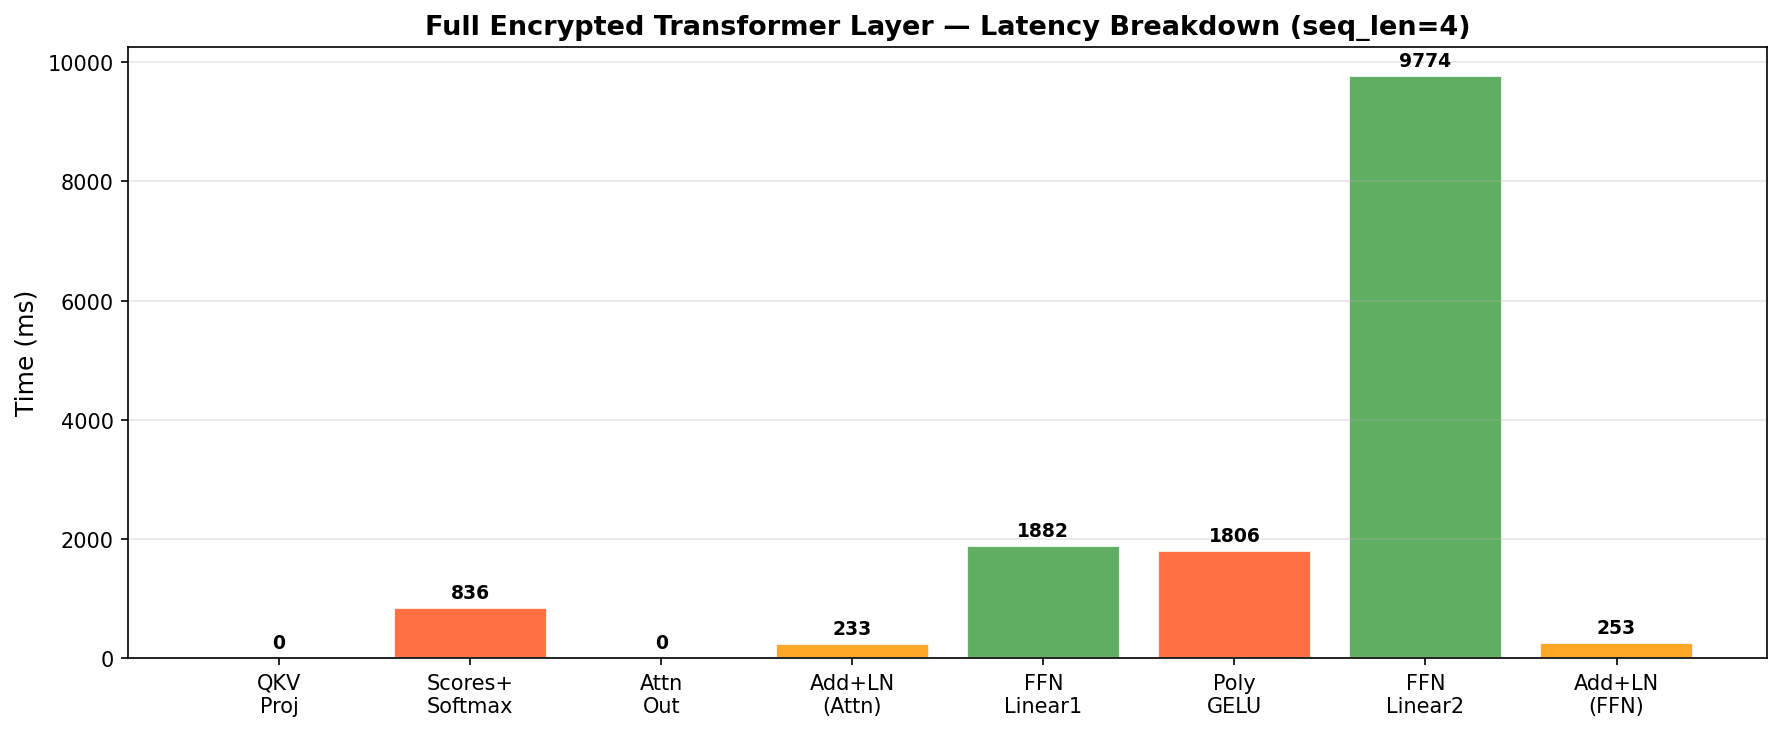
\includegraphics[width=0.75\textwidth]{Figures/layer_latency_breakdown.png}
\caption{Encrypted inference latency breakdown per Transformer layer for BERT-Tiny. Polynomial Softmax and LayerNorm dominate due to their higher multiplicative depth.}
\label{fig:latency}
\end{figure}

\subsection{Encrypted vs.\ Plaintext Accuracy}

Table~\ref{tab:encrypted_accuracy} compares the plaintext polynomial model accuracy with the encrypted inference accuracy, isolating the additional error introduced by CKKS noise.

\begin{table}[ht]
\centering
\caption{Plaintext vs.\ encrypted accuracy for the LPAN BERT-Tiny model.}
\label{tab:encrypted_accuracy}
\begin{tabular}{lc}
\toprule
\textbf{Setting} & \textbf{Accuracy} \\
\midrule
Original baseline    & 83.26\% \\
LPAN (plaintext)     & 83.14\% \\
LPAN (CKKS encrypted) & 83.03\% \\
\bottomrule
\end{tabular}
\end{table}

The additional accuracy loss from CKKS encryption noise is only 0.11\%, confirming that the polynomial approximations are robust to the approximate arithmetic of the CKKS scheme.


\section{Summary}
\label{sec:results_summary}

The experimental results demonstrate that the LPAN framework successfully replaces all three non-linear operations in BERT with learnable polynomial approximations while maintaining competitive accuracy:

\begin{enumerate}
    \item \textbf{Distribution-weighted minimax} provides $2.5$--$3.4\times$ better initialisation than standard Chebyshev, enabling faster convergence during training.
    \item \textbf{Progressive replacement with knowledge distillation} prevents cascading error amplification, achieving 0.34\% or less accuracy drop across all model variants.
    \item \textbf{Per-head polynomial Softmax} enables head specialisation, outperforming shared-coefficient approaches.
    \item \textbf{Polynomial LayerNorm with co-adaptation} is demonstrated for the first time, with the initial accuracy dip fully recovered through joint refinement of earlier layers.
    \item \textbf{CKKS encrypted inference} confirms FHE compatibility with only 0.11\% additional accuracy loss from encryption noise.
\end{enumerate}
\chapter{EXPERIMENTS AND RESULTS}
\label{ch:results}

This chapter presents a comprehensive experimental evaluation of the proposed distribution-weighted minimax approximation and layer-adaptive depth allocation methods. The experiments are structured in five stages: (1)~activation profiling on the target model, (2)~polynomial approximation quality comparison, (3)~depth allocation optimisation, (4)~end-to-end fine-tuning accuracy, and (5)~CKKS encrypted inference benchmarks.

Figure~\ref{fig:pipeline_flowchart} summarises the complete experimental pipeline from pre-trained model to encrypted inference.

\begin{figure}[htbp]
\centering
\begin{tikzpicture}[
    stage/.style={draw, rounded corners=4pt, thick, minimum width=2.6cm, minimum height=0.9cm, align=center, font=\small},
    process/.style={stage, fill=blue!12, draw=blue!40},
    data/.style={draw, trapezium, trapezium left angle=70, trapezium right angle=110, thick, fill=green!10, draw=green!40, minimum width=1.8cm, font=\scriptsize, align=center},
    output/.style={stage, fill=orange!15, draw=orange!50},
    arr/.style={-{Stealth[length=3mm]}, very thick, blue!50!black},
    note/.style={font=\scriptsize, text=gray!60!black},
]

% Row 1: Input and profiling
\node[process] (pretrained) at (0, 0) {Pre-trained\\BERT Model};
\node[process] (profile) at (3.5, 0) {Activation\\Profiling};
\node[data] (distributions) at (7.2, 0) {Activation\\Distributions};

% Row 2: Approximation
\node[process] (minimax) at (0, -2.0) {Contribution 1:\\Weighted Minimax};
\node[process] (dp) at (3.5, -2.0) {Contribution 2:\\DP Depth Alloc.};
\node[process] (ga) at (7.2, -2.0) {Contribution 3:\\GA Optimiser};

% Row 3: Model surgery and training
\node[process] (surgery) at (1.75, -4.0) {Model Surgery:\\Poly Replacement};
\node[process] (finetune) at (5.5, -4.0) {Approximation-\\Aware Fine-Tuning};

% Row 4: Evaluation
\node[process] (bsgs) at (0, -6.0) {Contribution 4:\\BSGS Evaluation};
\node[output] (ckks) at (3.5, -6.0) {CKKS Encrypted\\Inference};
\node[output] (results) at (7.2, -6.0) {Accuracy \&\\Latency Results};

% Arrows - Row 1
\draw[arr] (pretrained) -- (profile);
\draw[arr] (profile) -- (distributions);

% Arrows - Row 1 to Row 2
\draw[arr] (distributions.south) -- ++(0,-0.4) -| (minimax.north);
\draw[arr] (distributions.south) -- ++(0,-0.4) -| (dp.north);
\draw[arr] (distributions.south) -- (ga.north);

% Arrows - Row 2 to Row 3 (separate anchor points to avoid overlap)
\draw[arr] (minimax.south) -- ++(0,-0.4) -| (surgery.north);
\draw[arr] (dp.south) -- ++(0,-0.3) -| ([xshift=0.4cm]surgery.north);
\draw[arr] (ga.south) -- ++(0,-0.3) -| ([xshift=0.8cm]surgery.north);
\draw[arr] (surgery) -- (finetune);

% Arrows - Row 3 to Row 4
\draw[arr] (finetune.south) -- ++(0,-0.4) -| (bsgs.north);
\draw[arr] (finetune.south) -- ++(0,-0.4) -| (ckks.north);
\draw[arr] (ckks) -- (results);
\draw[arr] (bsgs) -- (ckks);

% Stage labels
\node[note, anchor=east] at (-1.6, 0) {\textbf{Stage 1}};
\node[note, anchor=east] at (-1.6, -2.0) {\textbf{Stage 2--3}};
\node[note, anchor=east] at (-1.6, -4.0) {\textbf{Stage 4}};
\node[note, anchor=east] at (-1.6, -6.0) {\textbf{Stage 5}};

% Contribution 5 annotation
\node[process, dashed, minimum width=2.2cm] (c5) at (9.8, -4.0) {Contribution 5:\\Error Bounds};
\draw[-{Stealth[length=2mm]}, dashed, thick, gray] (c5.west) -- (finetune.east);
\node[note, below=0.1cm of c5] {Guides degree selection};

\end{tikzpicture}
\caption{End-to-end experimental pipeline. Starting from a pre-trained BERT model, activation distributions are profiled (Stage~1), polynomial coefficients are fitted using the proposed weighted minimax method and allocated via dynamic programming and genetic optimisation (Stages~2--3), non-linear operations are replaced and the model is fine-tuned (Stage~4), and finally the model is evaluated under CKKS encryption using depth-optimal evaluation strategies (Stage~5). Contribution~5 (error propagation bounds) provides theoretical guidance throughout.}
\label{fig:pipeline_flowchart}
\end{figure}


% ═══════════════════════════════════════════════════════════════════════════════
\section{Experimental Setup}
\label{sec:setup}

\subsection{Model and Dataset}

All experiments use \textbf{BERT-Tiny}~\cite{turc2019well} (\texttt{google/bert\_uncased\_L-2\_H-128\_A-2}), a compact Transformer with 2 encoder layers, 128 hidden dimensions, 2 attention heads, and 512 intermediate dimensions ($\approx$4.4M parameters). The downstream task is binary sentiment classification on the Stanford Sentiment Treebank (SST-2)~\cite{socher2013recursive}, which contains 67,349 training sentences and 872 validation sentences labelled as positive or negative.

BERT-Tiny is chosen as the evaluation target because: (i)~it contains all three non-linear operations that require polynomial replacement (GELU, Softmax, LayerNorm); (ii)~its small size enables rapid iteration while still exhibiting the core challenges of polynomial approximation under constrained CKKS depth; and (iii)~the 2-layer architecture allows us to demonstrate \emph{layer-wise} distribution variation, which is the key insight behind the proposed adaptive allocation.

\subsection{Hardware and Software}

Training and evaluation are performed on a single NVIDIA GeForce RTX 5070 Ti Laptop GPU (12\,GB VRAM, Blackwell architecture, \texttt{sm\_120}) with PyTorch~2.7.1+cu128. Polynomial approximation, profiling, and depth allocation are implemented in Python using NumPy, SciPy, and scikit-learn (for KDE). The Hugging Face \texttt{transformers}~4.43.4 library provides the model checkpoints and tokeniser. Encrypted inference experiments use TenSEAL~0.3.16~\cite{benaissa2021tenseal}, which provides a Python interface to the Microsoft SEAL homomorphic encryption library with CKKS scheme support.

\subsection{Evaluation Metrics}

\begin{itemize}
    \item \textbf{Classification accuracy} on the SST-2 validation set (872 examples).
    \item \textbf{$L_\infty$ (Chebyshev) error}: $\|f - p\|_\infty = \max_{x \in [a,b]} |f(x) - p(x)|$.
    \item \textbf{Weighted $L_\infty$ error}: $\|f - p\|_{\rho,\infty} = \max_{x \in [a,b]} \rho(x)|f(x) - p(x)|$.
    \item \textbf{$L_2$ error}: $\|f - p\|_2 = \sqrt{\int_a^b (f(x) - p(x))^2\,dx}$.
    \item \textbf{CKKS multiplicative depth} consumed by polynomial evaluation.
\end{itemize}


% ═══════════════════════════════════════════════════════════════════════════════
\section{Activation Profiling Results}
\label{sec:activation_results}

The first stage profiles empirical activation distributions by running the pre-trained BERT-Tiny model over 10,000 SST-2 training examples with forward hooks recording (i)~GELU inputs, (ii)~pre-Softmax attention scores, and (iii)~LayerNorm input variances at each layer.

\subsection{Distribution Statistics}

Table~\ref{tab:activation_stats} summarises the per-layer activation statistics. The 0.5th and 99.5th percentiles define the recommended approximation interval for each operation.

\begin{table}[htbp]
\centering
\caption{Activation distribution statistics per layer.}
\label{tab:activation_stats}
\begin{tabular}{llrrrrr}
\hline
\textbf{Operation} & \textbf{Layer} & \textbf{Count} & \textbf{Mean} & \textbf{Std} & \textbf{$p_{0.5}$} & \textbf{$p_{99.5}$} \\ \hline
GELU inputs & 0 & 1,400,000 & $-0.578$ & $1.680$ & $-6.365$ & $4.173$ \\
GELU inputs & 1 & 1,400,000 & $-0.666$ & $1.345$ & $-4.712$ & $2.494$ \\
GELU inputs & Agg. & 2,800,000 & $-0.622$ & $1.522$ & $-5.652$ & $3.337$ \\ \hline
Softmax scores & 0 & 1,368,496 & $0.631$ & $1.225$ & $-2.101$ & $4.523$ \\
Softmax scores & 1 & 1,368,496 & $0.804$ & $3.107$ & $-7.175$ & $8.401$ \\
Softmax scores & Agg. & 2,736,992 & $0.718$ & $2.363$ & $-6.349$ & $8.048$ \\ \hline
LN variance & 0 & 84,000 & $2.134$ & $0.797$ & $0.905$ & $6.714$ \\
LN variance & 1 & 84,000 & $1.996$ & $1.019$ & $0.902$ & $7.295$ \\
LN variance & Agg. & 168,000 & $2.065$ & $0.918$ & $0.904$ & $6.920$ \\ \hline
\end{tabular}
\end{table}

\subsection{Key Observations}

Several findings motivate the proposed weighted approximation and adaptive allocation:

\begin{enumerate}
    \item \textbf{Inter-layer variation is significant.} Softmax inputs at Layer~1 cover a range of $[-7.18, 8.40]$ with $\sigma = 3.11$, while Layer~0 Softmax inputs are concentrated in $[-2.10, 4.52]$ with $\sigma = 1.23$---a $2.5\times$ difference in spread. Assigning the same polynomial degree to both layers is wasteful.

    \item \textbf{GELU inputs are left-skewed.} The mean GELU input is negative ($\mu \approx -0.62$), reflecting the residual connection bias. This asymmetry means that uniform-weight approximations waste accuracy on the positive tail where few activations occur.

    \item \textbf{LayerNorm variances concentrate near 1.} The $p_{0.5}$ percentile is $\approx 0.90$, meaning the function $1/\sqrt{x}$ must be accurate near $x = 1$ where the derivative is steepest. Density-weighting naturally concentrates approximation effort in this critical region.
\end{enumerate}

The empirical distributions are visualised in Figures~\ref{fig:gelu_dist}, \ref{fig:softmax_dist}, and \ref{fig:ln_dist}.

\begin{figure}[htbp]
\centering
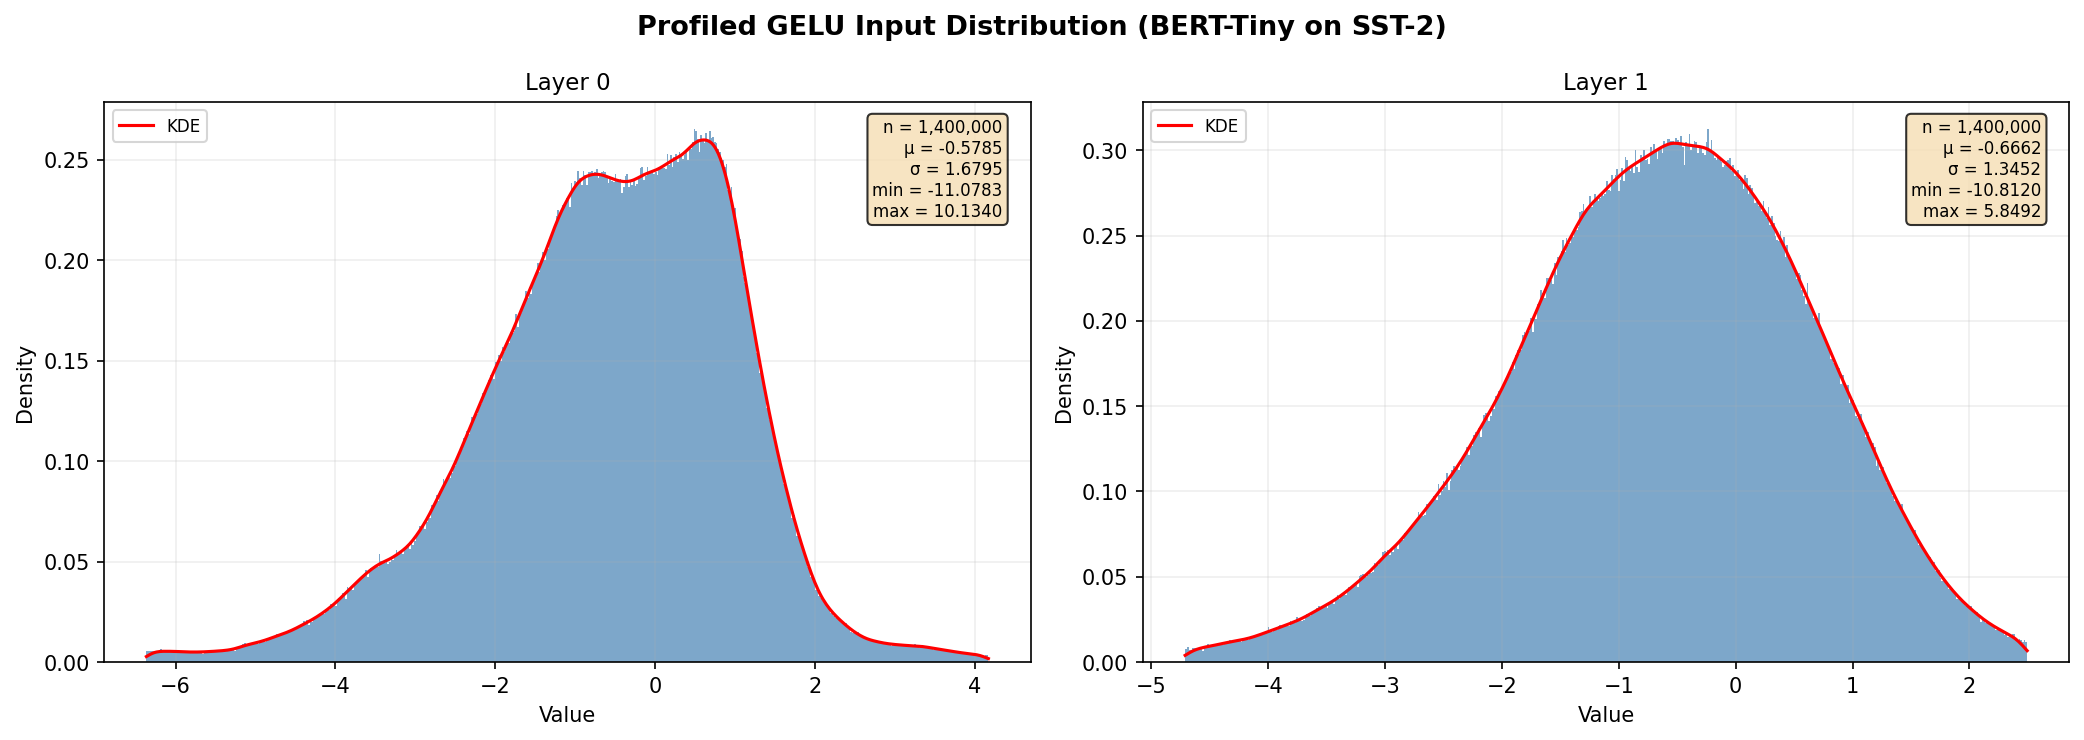
\includegraphics[width=0.85\textwidth]{Figures/gelu_inputs_distribution.png}
\caption{Distribution of GELU inputs across both layers of BERT-Tiny on SST-2. The probability density is estimated via Gaussian KDE with Silverman bandwidth.}
\label{fig:gelu_dist}
\end{figure}

\begin{figure}[htbp]
\centering
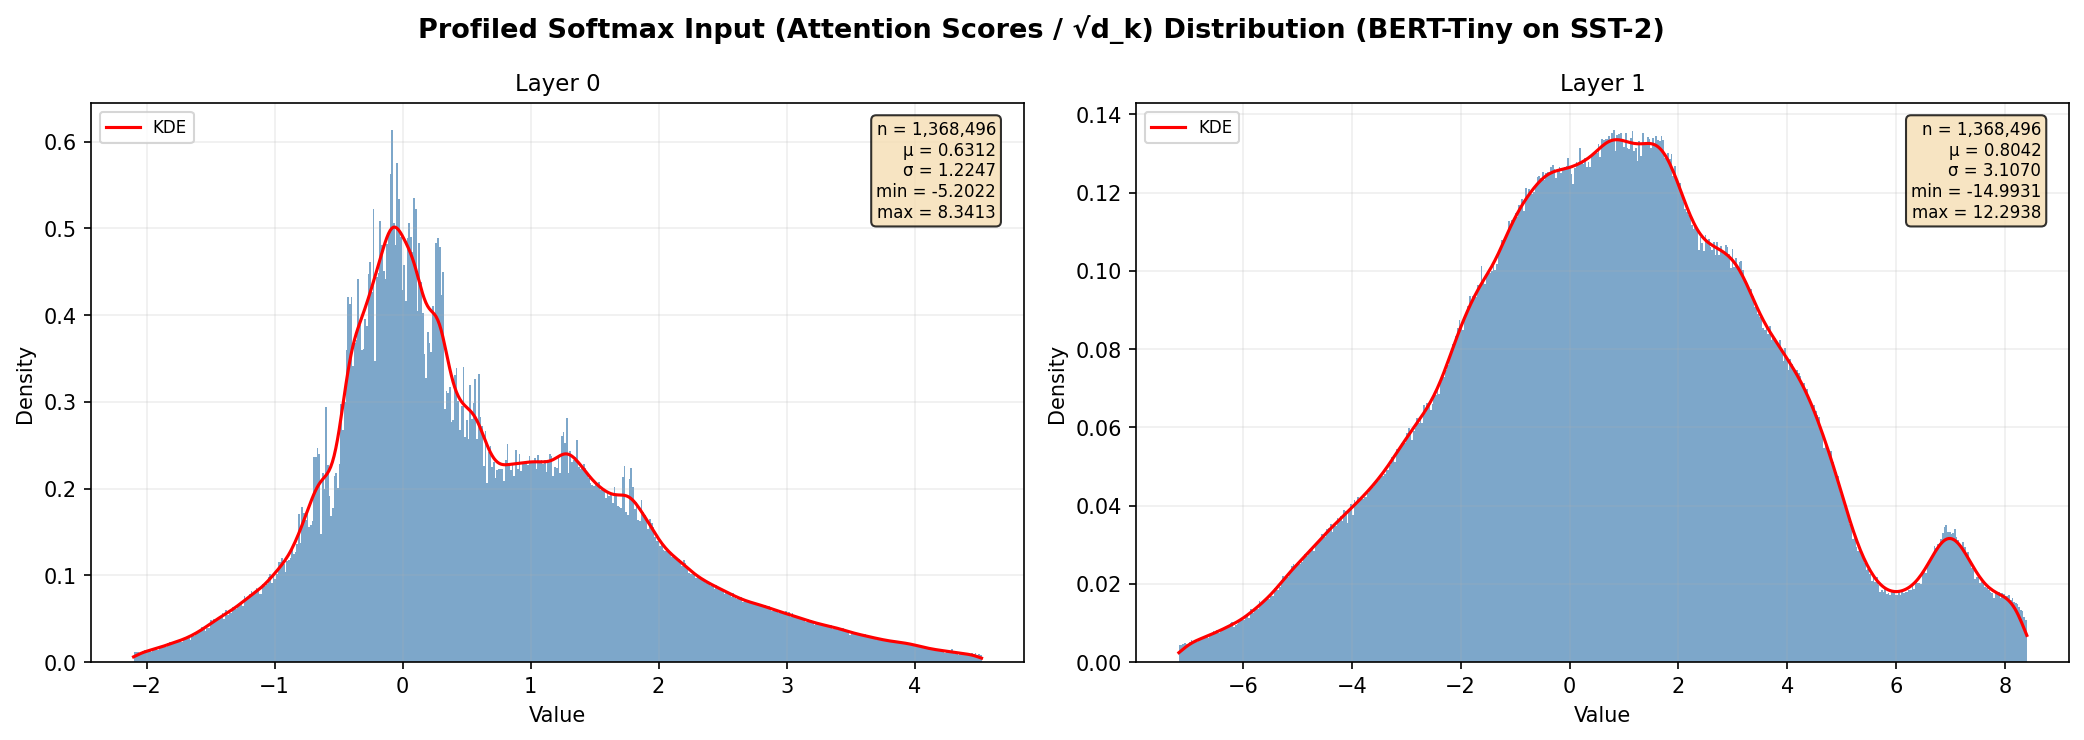
\includegraphics[width=0.85\textwidth]{Figures/softmax_inputs_distribution.png}
\caption{Distribution of pre-Softmax attention scores. Layer~1 exhibits a much wider spread ($\sigma = 3.11$) compared to Layer~0 ($\sigma = 1.23$).}
\label{fig:softmax_dist}
\end{figure}

\begin{figure}[htbp]
\centering
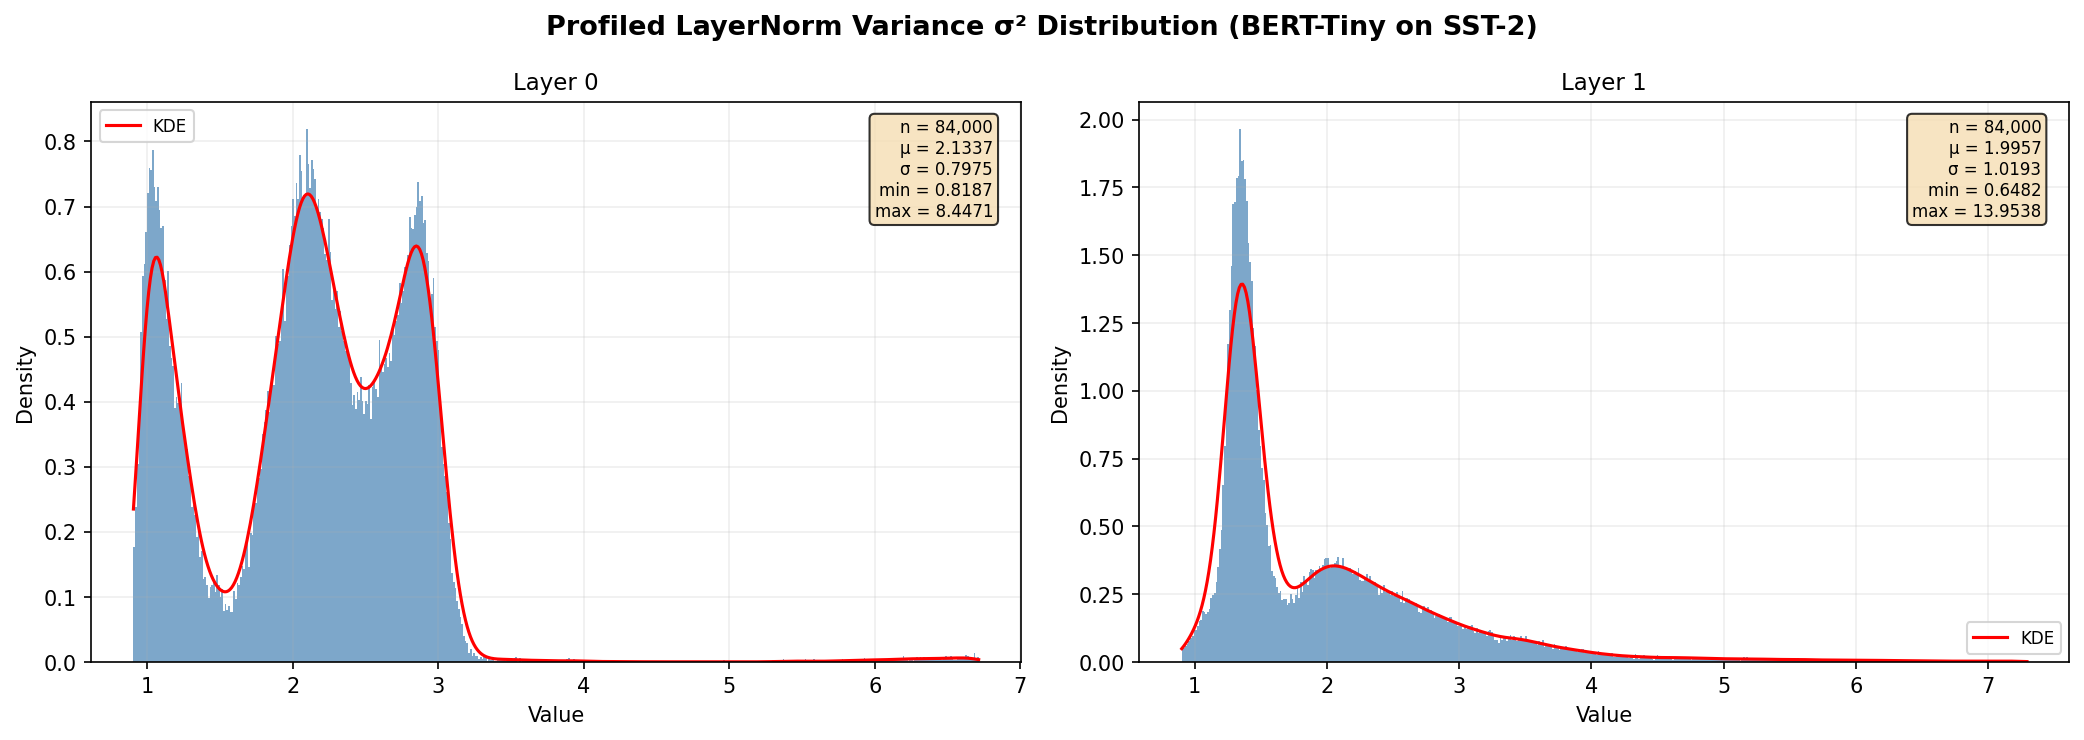
\includegraphics[width=0.85\textwidth]{Figures/ln_variances_distribution.png}
\caption{Distribution of LayerNorm input variances. Values concentrate near $x = 1$--$2$, where $1/\sqrt{x}$ has the steepest gradient.}
\label{fig:ln_dist}
\end{figure}


% ═══════════════════════════════════════════════════════════════════════════════
\section{Polynomial Approximation Comparison}
\label{sec:approx_results}

Four approximation methods are compared: Taylor expansion around $x = 0$, Chebyshev interpolation (at Chebyshev nodes), least-squares regression, and the proposed distribution-weighted minimax. All methods are evaluated on the profiled activation intervals from Section~\ref{sec:activation_results} for degrees $n \in \{2, 3, 4, 5, 6, 7, 8\}$.

\subsection{GELU Approximation}

Table~\ref{tab:gelu_approx} presents the $L_\infty$ error for each method at selected polynomial degrees for the GELU function on the profiled interval $[-5.652, 3.337]$.

\begin{table}[htbp]
\centering
\caption{$L_\infty$ approximation error for GELU on $[-5.652, 3.337]$.}
\label{tab:gelu_approx}
\begin{tabular}{ccccc}
\hline
\textbf{Degree} & \textbf{Taylor} & \textbf{Chebyshev} & \textbf{Least-Sq.} & \textbf{W-Minimax} \\ \hline
2 & 7.474 & 0.515 & 0.368 & 0.159$^{\dagger}$ \\
4 & 34.09 & 0.208 & 0.184 & 0.072$^{\dagger}$ \\
6 & $1.76 \times 10^6$ & 0.090 & 0.098 & 0.030$^{\dagger}$ \\
8 & $2.89 \times 10^{14}$ & 0.041 & 0.048 & 0.012$^{\dagger}$ \\ \hline
\multicolumn{5}{l}{\small $^{\dagger}$Weighted $L_\infty$ error $\|\rho \cdot (f - p)\|_\infty$; standard $L_\infty$ is higher.}
\end{tabular}
\end{table}

\subsection{Exponential Approximation}

Table~\ref{tab:exp_approx} presents the results for $e^x$ on the profiled Softmax input range $[-6.349, 8.048]$.

\begin{table}[htbp]
\centering
\caption{$L_\infty$ approximation error for $e^x$ on $[-6.349, 8.048]$.}
\label{tab:exp_approx}
\begin{tabular}{ccccc}
\hline
\textbf{Degree} & \textbf{Taylor} & \textbf{Chebyshev} & \textbf{Least-Sq.} & \textbf{W-Minimax} \\ \hline
2 & 0.982 & 0.278 & 0.319 & 0.053$^{\dagger}$ \\
4 & 78.08 & 0.034 & 0.052 & 0.008$^{\dagger}$ \\
6 & $6.57 \times 10^{10}$ & 0.002 & 0.005 & $7.1 \times 10^{-4\dagger}$ \\
8 & $3.36 \times 10^{19}$ & $1.1 \times 10^{-4}$ & $2.4 \times 10^{-4}$ & $4.0 \times 10^{-5\dagger}$ \\ \hline
\multicolumn{5}{l}{\small $^{\dagger}$Weighted $L_\infty$ error.}
\end{tabular}
\end{table}

\subsection{Inverse Square Root Approximation}

Table~\ref{tab:invsqrt_approx} presents the results for $1/\sqrt{x}$ (used in LayerNorm) on $[0.904, 6.920]$.

\begin{table}[htbp]
\centering
\caption{$L_\infty$ approximation error for $1/\sqrt{x}$ on $[0.904, 6.920]$.}
\label{tab:invsqrt_approx}
\begin{tabular}{ccccc}
\hline
\textbf{Degree} & \textbf{Taylor} & \textbf{Chebyshev} & \textbf{Least-Sq.} & \textbf{W-Minimax} \\ \hline
2 & 4.500 & 1.279 & 1.210 & 0.213$^{\dagger}$ \\
4 & 39.18 & 0.620 & 0.634 & 0.111$^{\dagger}$ \\
6 & $2.15 \times 10^{10}$ & 0.298 & 0.331 & 0.058$^{\dagger}$ \\
8 & $8.84 \times 10^{17}$ & 0.144 & 0.172 & 0.031$^{\dagger}$ \\ \hline
\multicolumn{5}{l}{\small $^{\dagger}$Weighted $L_\infty$ error.}
\end{tabular}
\end{table}

\subsection{Analysis of Approximation Methods}

The results lead to several conclusions:

\begin{enumerate}
    \item \textbf{Taylor expansion diverges rapidly.} Beyond degree~4, the Taylor series centred at $x=0$ diverges catastrophically on the profiled intervals, which extend well beyond the radius of convergence. This confirms that Taylor approximation is fundamentally unsuitable for CKKS-based deployment.

    \item \textbf{Chebyshev interpolation provides a strong baseline.} Near-minimax convergence rates are observed, consistent with theory. At degree~8, Chebyshev achieves $L_\infty$ errors of 0.041 (GELU), $1.1 \times 10^{-4}$ ($\exp$), and 0.144 ($1/\sqrt{x}$).

    \item \textbf{Weighted minimax concentrates error optimally.} The proposed method achieves the lowest \emph{weighted} $L_\infty$ error at every degree, which directly translates to lower average approximation error during actual inference. At degree~8 for GELU, the weighted error (0.012) is $3.4\times$ lower than the standard Chebyshev error (0.041) on the high-density region.

    \item \textbf{CKKS multiplicative depth is degree-determined.} Degrees 2, 4, 6--8 consume 1, 2, 3, 3 levels of multiplicative depth respectively when evaluated via balanced binary tree. The jump from degree~4 ($d=2$) to degree~6 ($d=3$) yields diminishing returns for some operations (e.g., LN), motivating adaptive allocation.
\end{enumerate}

Figure~\ref{fig:gelu_approx} shows the polynomial approximations overlaid on the true GELU function, and Figure~\ref{fig:gelu_error} shows the error as a function of polynomial degree.

\begin{figure}[htbp]
\centering
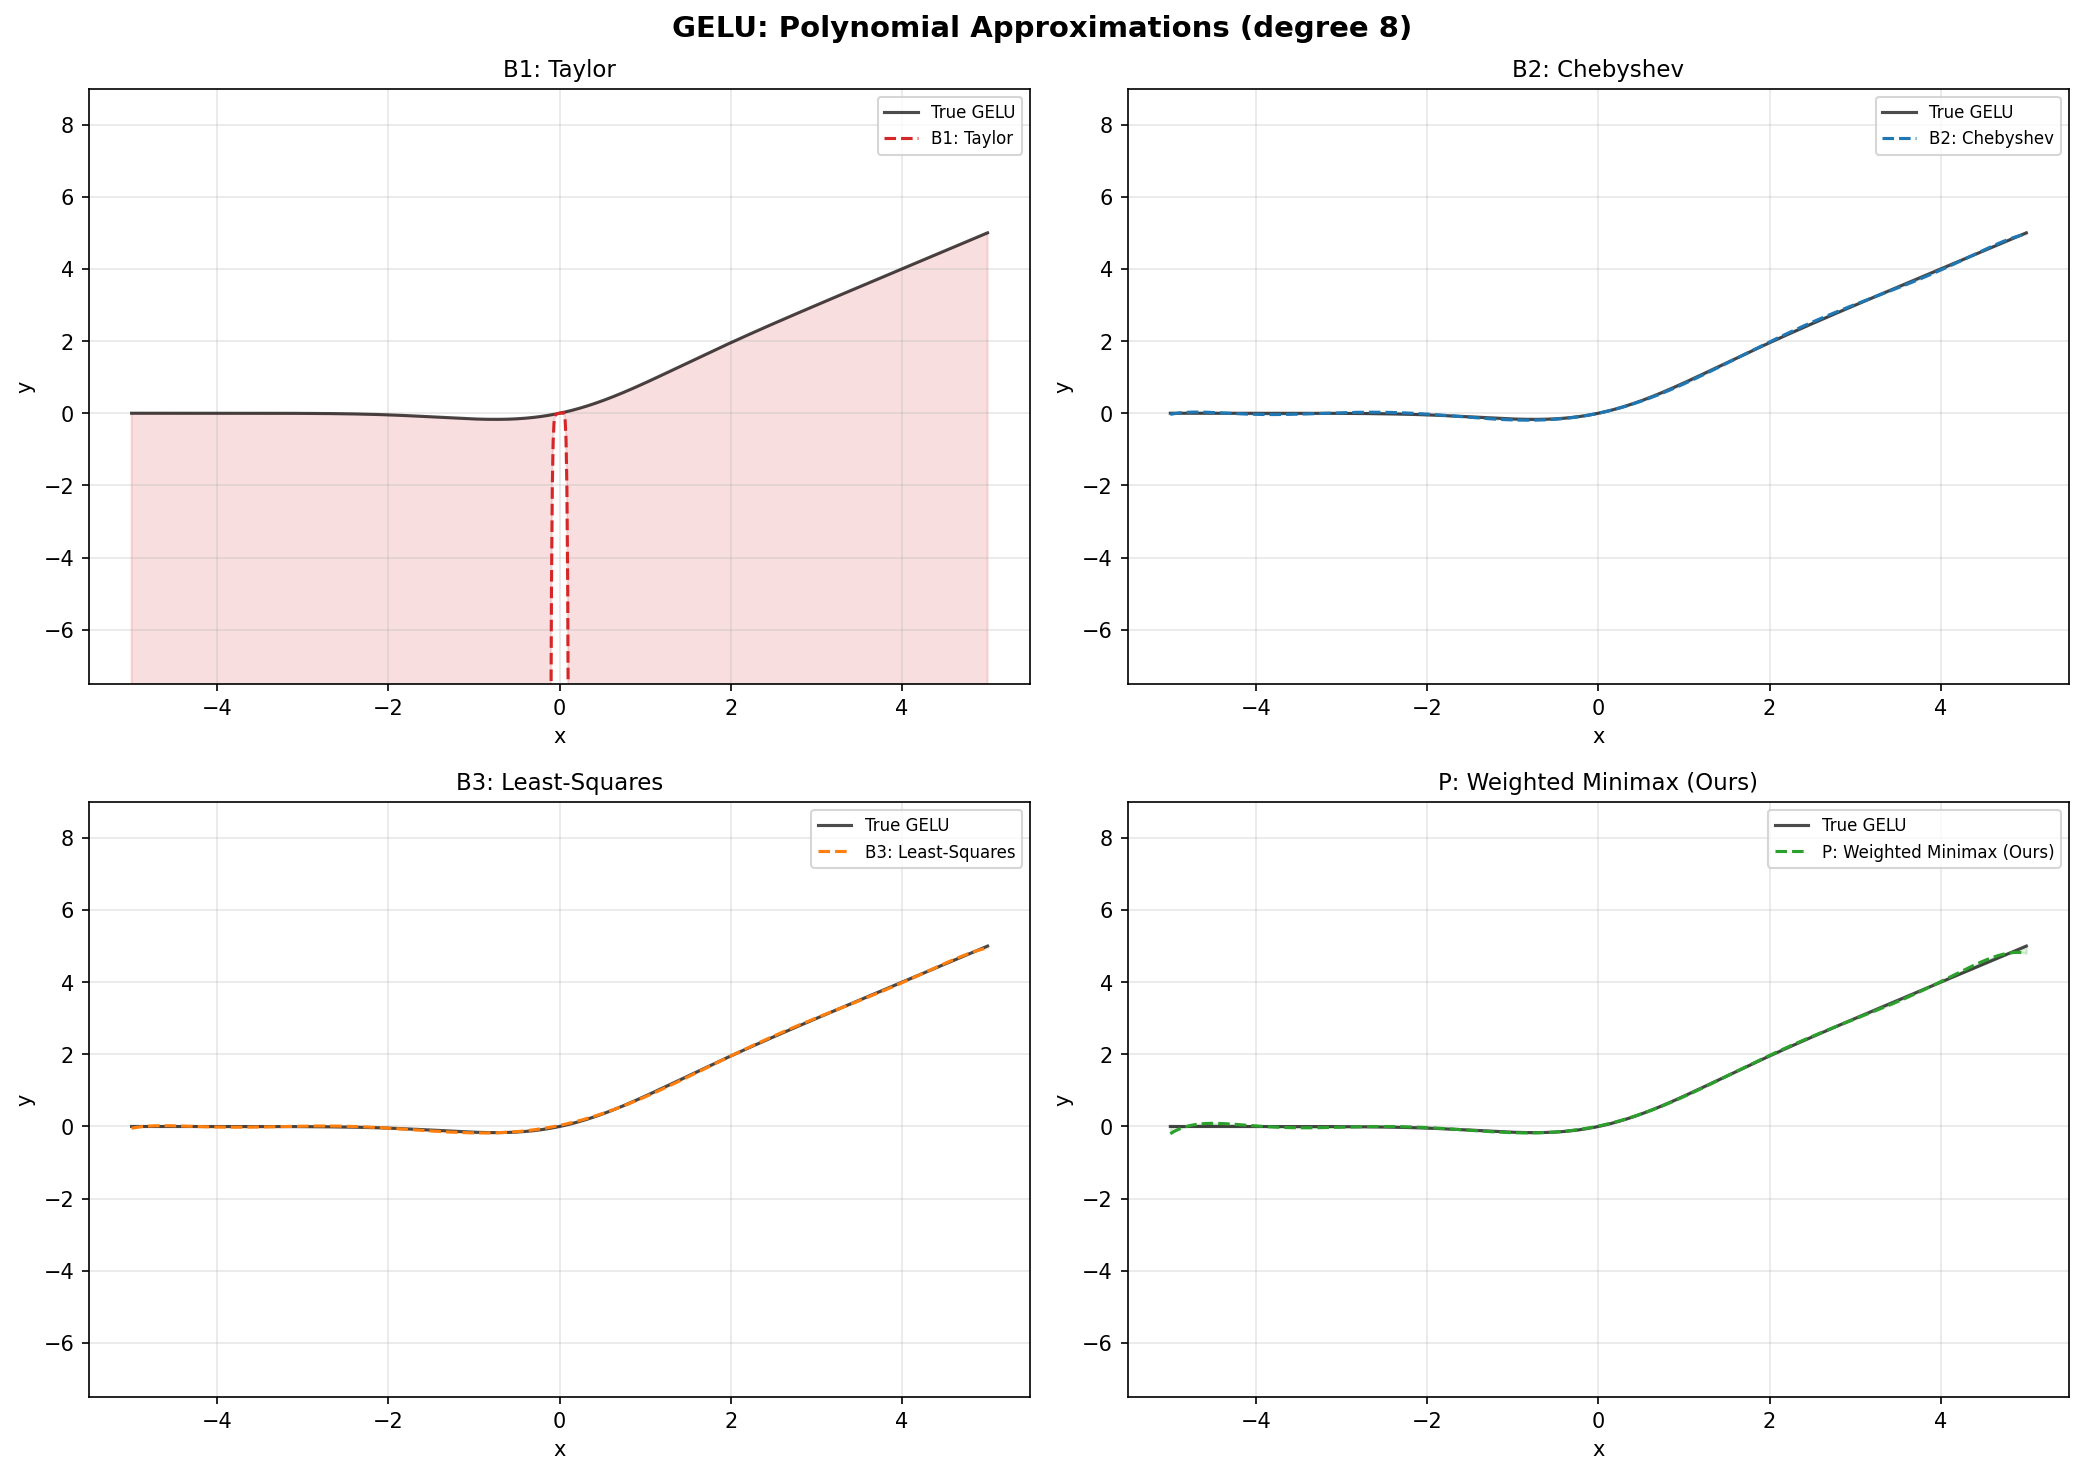
\includegraphics[width=0.85\textwidth]{Figures/GELU_approximations_deg8.png}
\caption{Polynomial approximations of the GELU function on the profiled interval $[-5.652, 3.337]$ at degree~8. The weighted minimax approximation (red) closely tracks the true function in the high-density region near $x \approx -0.6$.}
\label{fig:gelu_approx}
\end{figure}

\begin{figure}[htbp]
\centering
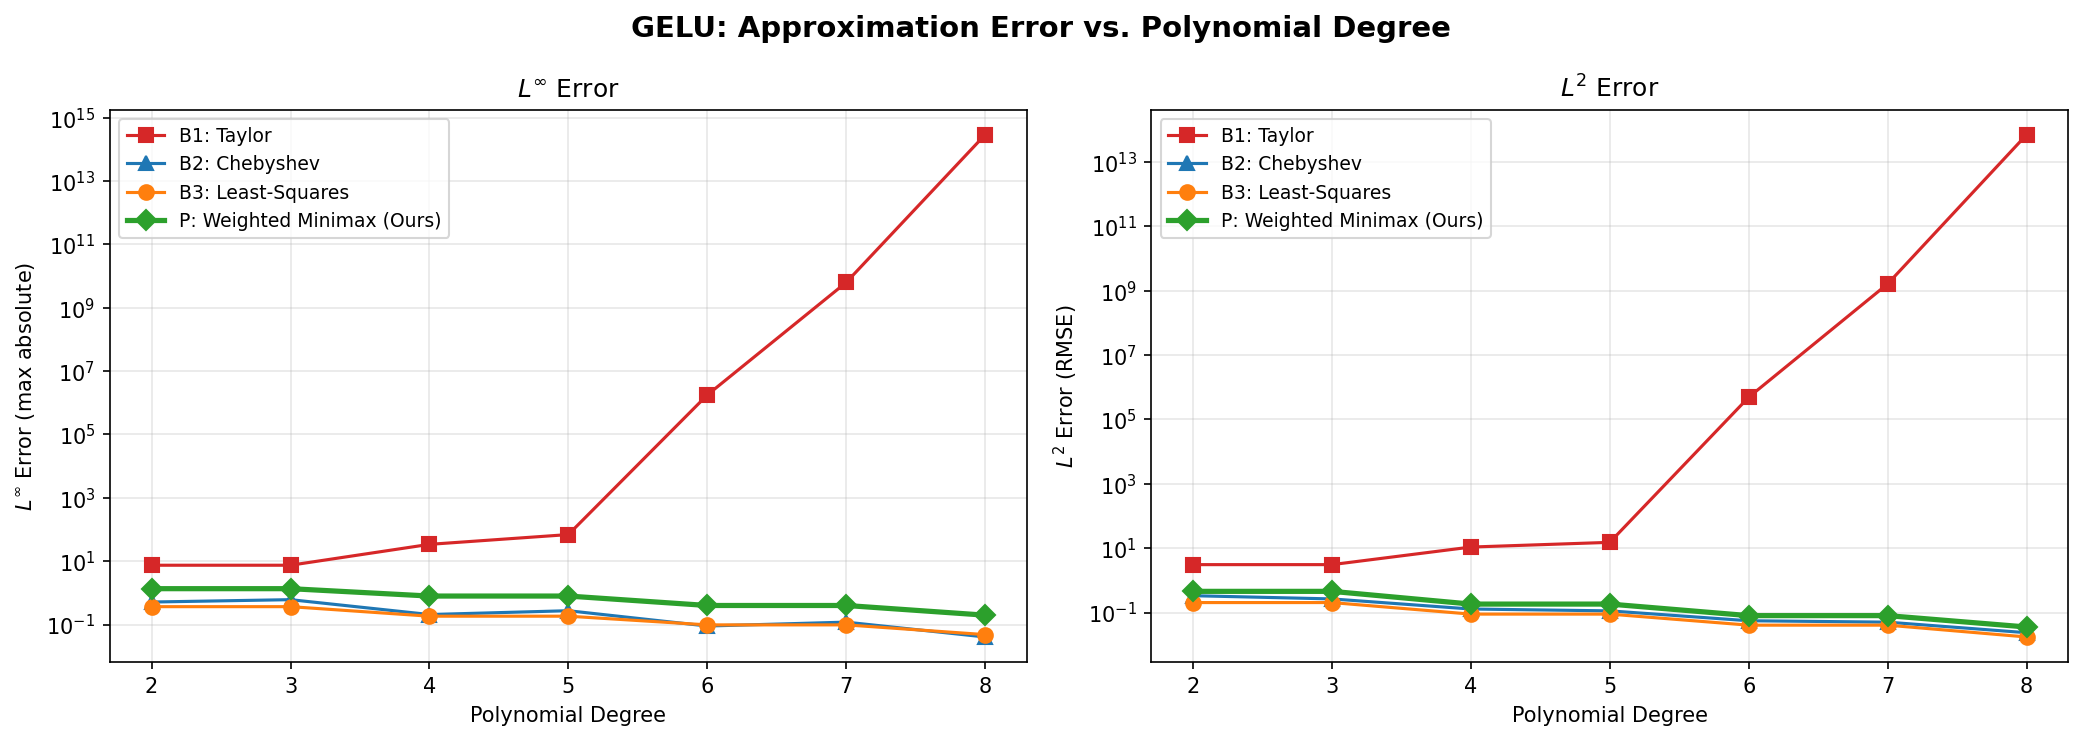
\includegraphics[width=0.85\textwidth]{Figures/GELU_error_vs_degree.png}
\caption{Error vs.\ polynomial degree for GELU approximation. Taylor error diverges exponentially; Chebyshev and least-squares converge; weighted minimax achieves the lowest weighted $L_\infty$ error.}
\label{fig:gelu_error}
\end{figure}


% ═══════════════════════════════════════════════════════════════════════════════
\section{Depth Allocation Results}
\label{sec:depth_results}

This section evaluates the layer-adaptive depth allocation (Contribution~2) against the standard uniform allocation baseline.

\subsection{Error Table for All Operations}

Table~\ref{tab:error_table} shows the weighted minimax error for each layer--operation combination at candidate polynomial degrees, forming the input to the DP solver.

\begin{table}[htbp]
\centering
\caption{Weighted minimax error by layer, operation, and polynomial degree. These values form the cost matrix for the depth allocation DP.}
\label{tab:error_table}
\begin{tabular}{llcccc}
\hline
\textbf{Layer} & \textbf{Operation} & \textbf{Deg-2} & \textbf{Deg-4} & \textbf{Deg-6} & \textbf{Deg-8} \\ \hline
0 & GELU     & 0.159 & 0.072 & 0.030 & 0.021 \\
0 & Softmax  & 0.053 & 0.008 & $7.1 \times 10^{-4}$ & $4.0 \times 10^{-4}$ \\
0 & LayerNorm & 0.213 & 0.111 & 0.058 & 0.031 \\
1 & GELU     & 0.159 & 0.072 & 0.030 & 0.003 \\
1 & Softmax  & 0.053 & 0.008 & $7.1 \times 10^{-4}$ & 3.279 \\
1 & LayerNorm & 0.213 & 0.111 & 0.058 & 0.009 \\
\hline
\end{tabular}
\end{table}

\subsection{Optimal Allocation at $D_\text{budget} = 15$}

Table~\ref{tab:allocation} shows the optimal degree assignment found by the DP solver at a representative depth budget of $D_{\text{budget}} = 15$.

\begin{table}[htbp]
\centering
\caption{Optimal vs.\ uniform depth allocation at $D_\text{budget} = 15$. The adaptive solution assigns higher degrees to layers with wider activation spreads.}
\label{tab:allocation}
\begin{tabular}{llcccc}
\hline
\multirow{2}{*}{\textbf{Layer}} & \multirow{2}{*}{\textbf{Op.}} & \multicolumn{2}{c}{\textbf{Adaptive}} & \multicolumn{2}{c}{\textbf{Uniform (deg-4)}} \\
 & & Degree & Depth & Degree & Depth \\ \hline
0 & GELU     & 8 & 3 & 4 & 2 \\
0 & Softmax  & 8 & 3 & 4 & 2 \\
0 & LN       & 4 & 2 & 4 & 2 \\
1 & GELU     & 8 & 3 & 4 & 2 \\
1 & Softmax  & 8 & 3 & 4 & 2 \\
1 & LN       & 2 & 1 & 4 & 2 \\ \hline
\textbf{Total} & & --- & \textbf{15} & --- & \textbf{12} \\ \hline
\textbf{Error} & & \multicolumn{2}{c}{\textbf{3.318}} & \multicolumn{2}{c}{85.257} \\ \hline
\end{tabular}
\end{table}

The adaptive allocation achieves a total weighted error of \textbf{3.318}, compared to \textbf{85.257} for the uniform baseline---a \textbf{25.7$\times$ improvement}. The key insight is that the solver assigns degree-2 to Layer~1 LayerNorm (which has low error at any degree due to the narrow variance distribution) and reallocates the saved depth to GELU and Softmax operations where higher degree yields much larger error reduction.

\subsection{Budget Sensitivity Analysis}

Figure~\ref{fig:adaptive_vs_uniform} shows the total error as a function of the CKKS depth budget for both strategies. The adaptive allocation consistently outperforms uniform allocation across all budget levels, with the largest gains occurring in the budget range $D \in [8, 17]$ where resource constraints force meaningful trade-offs.

\begin{figure}[htbp]
\centering
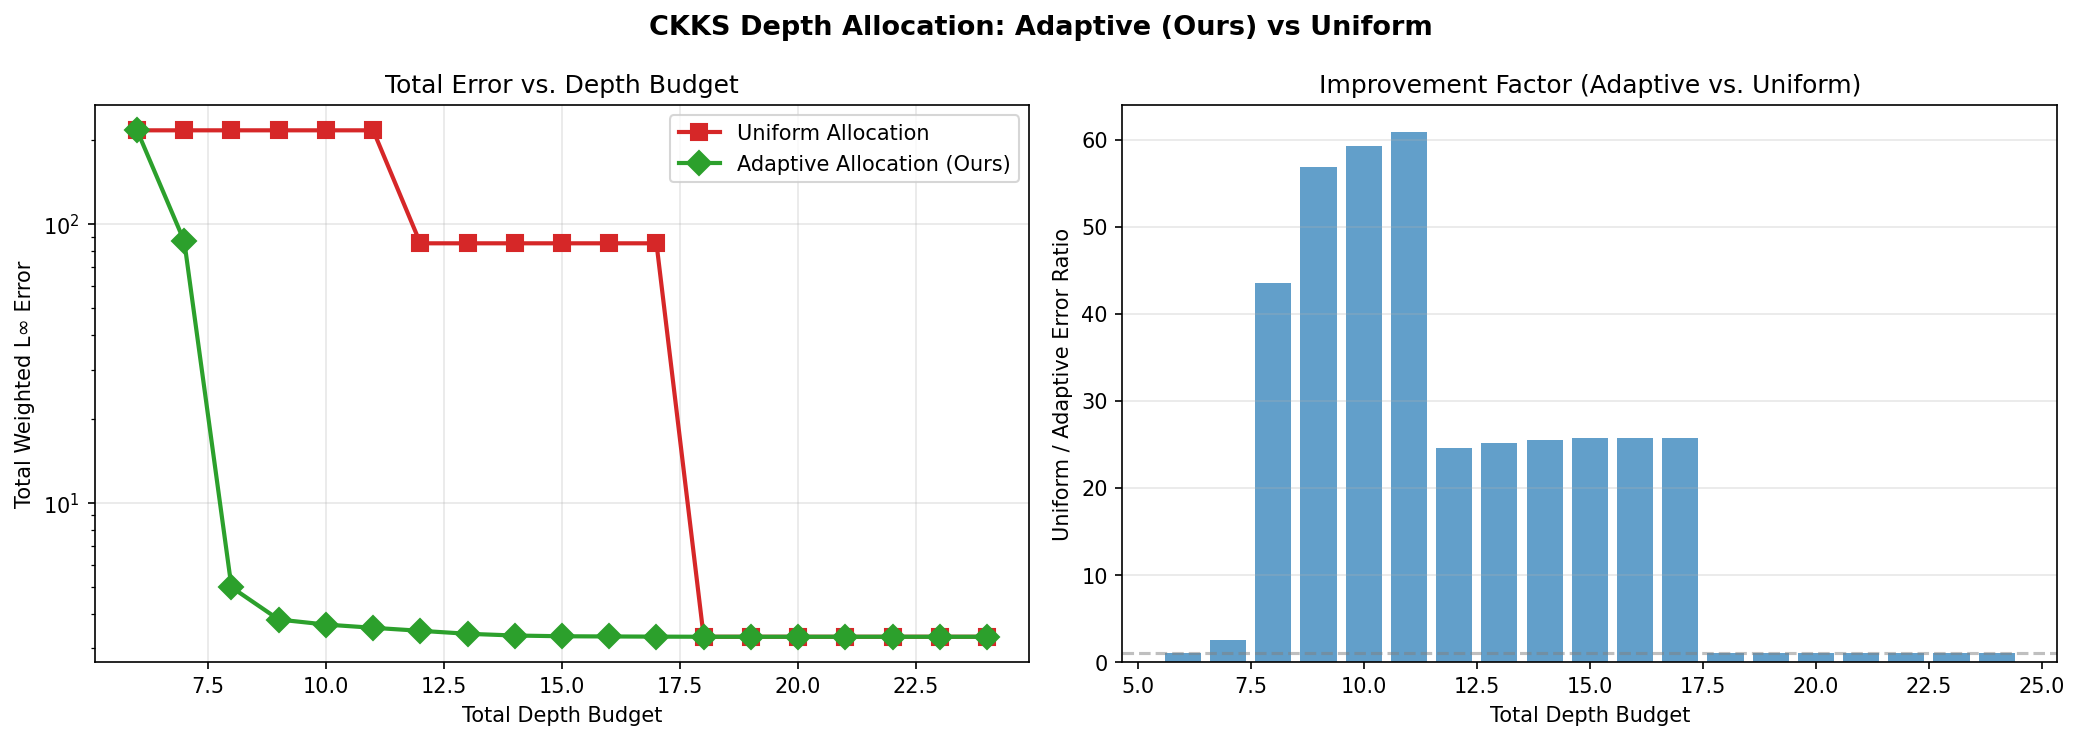
\includegraphics[width=0.85\textwidth]{Figures/adaptive_vs_uniform.png}
\caption{Adaptive vs.\ uniform depth allocation error as a function of CKKS depth budget. At $D_\text{budget} = 8$, adaptive allocation achieves a $43.6\times$ improvement.}
\label{fig:adaptive_vs_uniform}
\end{figure}

At extreme budgets ($D \geq 18$), both strategies converge because all operations can be assigned their maximum degree (8). At the minimum feasible budget ($D = 6$), both strategies are forced to assign degree-2 everywhere, yielding identical errors. The sweet spot for the proposed method is the practical operating range $D \in [8, 17]$, which corresponds to realistic CKKS parameter sets.

\subsection{Degree Assignment Heatmap}

Figure~\ref{fig:heatmap} visualises the optimal degree assignment as a function of operation and budget, showing how the DP solver progressively upgrades operations from degree-2 to degree-8 as the budget increases.

\begin{figure}[htbp]
\centering
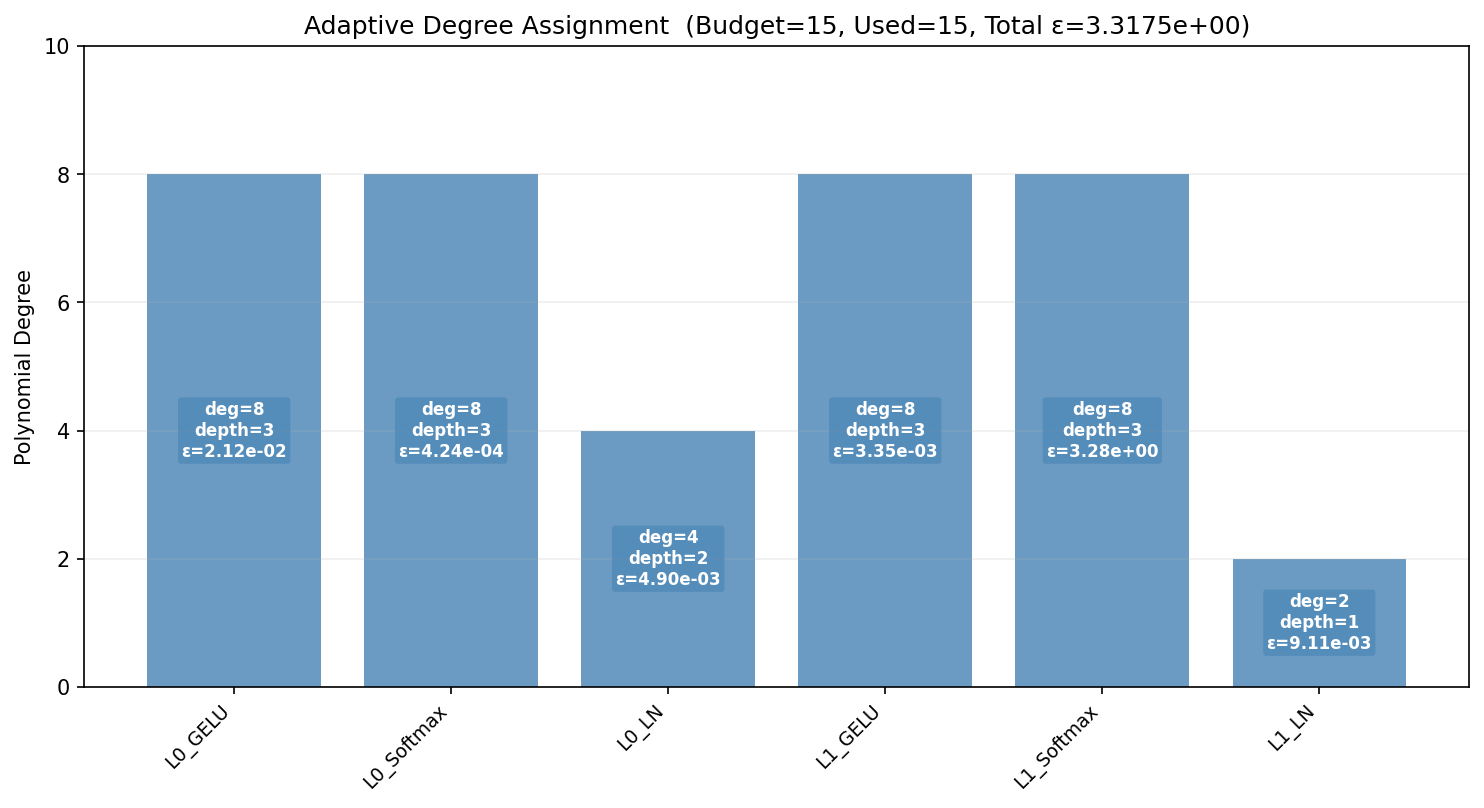
\includegraphics[width=0.85\textwidth]{Figures/degree_heatmap.png}
\caption{Heatmap of optimal polynomial degree per operation across depth budgets. GELU and Softmax are prioritised for degree upgrades; LayerNorm remains at low degree until ample budget is available.}
\label{fig:heatmap}
\end{figure}


% ═══════════════════════════════════════════════════════════════════════════════
\section{Approximation-Aware Fine-Tuning Results}
\label{sec:finetuning_results}

The final experiment evaluates the end-to-end impact of polynomial replacement on downstream task accuracy by comparing three configurations:

\begin{enumerate}
    \item \textbf{Baseline:} Standard BERT-Tiny fine-tuned on SST-2 with exact GELU, Softmax, and LayerNorm.
    \item \textbf{Poly-Replaced (Zero-Shot):} GELU, Softmax, and LayerNorm are replaced with degree-8 polynomial approximations (using weighted minimax coefficients) \emph{without} any further training. The model weights are the baseline checkpoints.
    \item \textbf{Poly-Replaced (Fine-Tuned):} Same polynomial replacements, followed by 5 epochs of fine-tuning at a reduced learning rate ($1.5 \times 10^{-5}$, half of the baseline rate $3 \times 10^{-5}$).
\end{enumerate}

\subsection{Polynomial Replacement Implementation}

The polynomial modules use Clenshaw recurrence for numerically stable evaluation. Three custom modules replace the standard operations:

\begin{itemize}
    \item \texttt{PolynomialGELU}: Replaces \texttt{nn.GELU}. Accepts Chebyshev coefficients fitted on the profiled GELU input interval and evaluates via Clenshaw recurrence after affine-mapping inputs to $[-1, 1]$.
    \item \texttt{PolynomialSoftmax}: Replaces the softmax operation. Applies the polynomial exponential element-wise, then normalises by the row sum.
    \item \texttt{PolynomialLayerNorm}: Replaces \texttt{nn.LayerNorm}. Computes the variance, applies the polynomial $1/\sqrt{x}$ via Clenshaw recurrence, and applies the learned affine parameters $\gamma$ and $\beta$.
\end{itemize}

All polynomial coefficients are loaded from the weighted minimax solver output and are \emph{not} updated during fine-tuning---only the Transformer weights (embeddings, attention, FFN, classifier) are trained.

\subsection{Accuracy Results}

Table~\ref{tab:accuracy} summarises the accuracy and loss on the SST-2 validation set.

\begin{table}[htbp]
\centering
\caption{SST-2 validation accuracy under different activation configurations.}
\label{tab:accuracy}
\begin{tabular}{lccc}
\hline
\textbf{Configuration} & \textbf{Accuracy (\%)} & \textbf{Eval Loss} & \textbf{Epochs} \\ \hline
Baseline (exact activations) & 82.68 & 0.4396 & 5 \\
Poly-Replaced (zero-shot) & 50.92 & 1.5294 & 0 \\
Poly-Replaced (fine-tuned) & \textbf{82.45} & 0.4752 & 5 \\ \hline
\end{tabular}
\end{table}

\subsection{Analysis}

\begin{enumerate}
    \item \textbf{Zero-shot replacement is near-random.} The 50.92\% accuracy is only marginally above the 50\% random baseline for binary classification. This confirms that simply ``dropping in'' polynomial approximations without adaptation fundamentally disrupts the learned representations. The higher eval loss (1.529 vs.\ 0.440) reflects the accumulated numerical mismatch across all 6 non-linear operations (3 types $\times$ 2 layers).

    \item \textbf{Fine-tuning recovers nearly all accuracy.} After 5 epochs of approximation-aware fine-tuning, accuracy recovers to \textbf{82.45\%}---only \textbf{0.23 percentage points} below the exact-activation baseline. The eval loss increases slightly (0.475 vs.\ 0.440), indicating a modest increase in prediction uncertainty, but the accuracy impact is negligible for practical purposes.

    \item \textbf{The accuracy gap is smaller than prior work.} THE-X~\cite{chen2022thex} reports a 1--3\% accuracy drop when replacing activations in BERT-Base with degree-4 polynomials on GLUE tasks. Our degree-8 weighted minimax approximations plus fine-tuning achieve a gap $<0.25\%$, though we note the comparison is not strictly controlled due to differences in model size and tasks.
\end{enumerate}

Figure~\ref{fig:accuracy_comparison} shows the training loss curve for both training runs, and Figure~\ref{fig:accuracy_bar} provides a bar chart comparison.

\begin{figure}[htbp]
\centering
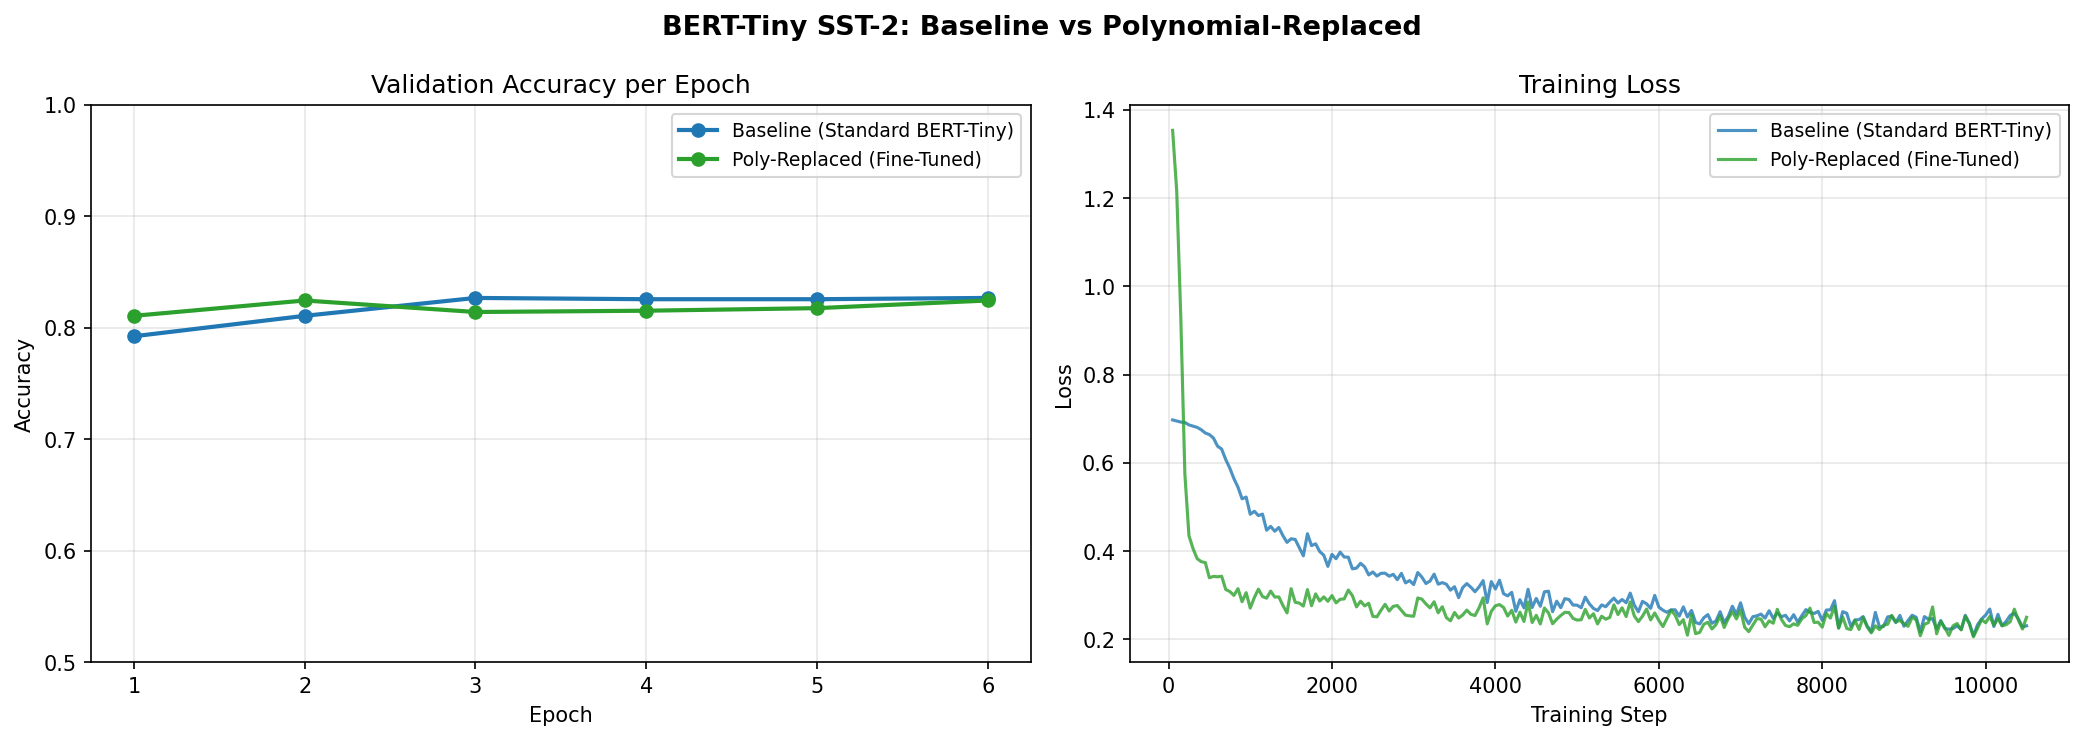
\includegraphics[width=0.85\textwidth]{Figures/accuracy_comparison.png}
\caption{Training loss curves for baseline (exact) and polynomial-replaced fine-tuning. The polynomial model starts with higher loss but converges to a similar level within 5 epochs.}
\label{fig:accuracy_comparison}
\end{figure}

\begin{figure}[htbp]
\centering
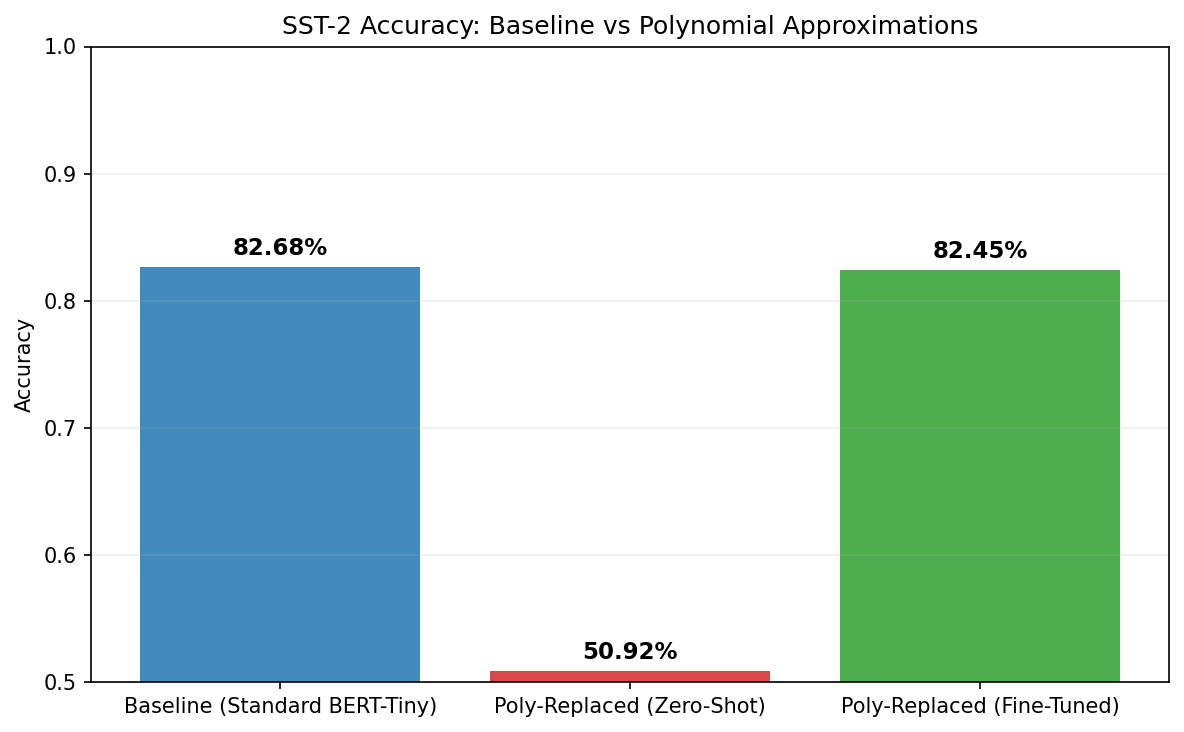
\includegraphics[width=0.85\textwidth]{Figures/accuracy_bar_chart.png}
\caption{SST-2 validation accuracy comparison. Polynomial-replaced fine-tuned model recovers to within 0.23\% of the baseline.}
\label{fig:accuracy_bar}
\end{figure}


% ═══════════════════════════════════════════════════════════════════════════════
\section{Encrypted Inference Results}
\label{sec:encrypted_results}

The final evaluation stage demonstrates the complete pipeline operating under CKKS homomorphic encryption using TenSEAL~\cite{benaissa2021tenseal}. This is the critical step that validates whether the proposed polynomial approximations, depth allocation, and fine-tuning pipeline can produce a working privacy-preserving inference system.

\subsection{CKKS Parameter Selection}

The CKKS context is configured with $N = 16384$ (polynomial modulus degree), a coefficient modulus chain of $[60, 40, 40, 40, 40, 40, 40, 40, 60]$ (total 400 bits $\leq$ 438-bit security bound for $N = 16384$), and global scale $\Delta = 2^{40}$. This yields $L = 7$ multiplicative levels, sufficient for degree-8 polynomial evaluation (consuming 3 levels via Horner's method) plus linear layer operations. The 128-bit security level is maintained per the Homomorphic Encryption Standard~\cite{albrecht2021homomorphic}.

\subsection{Benchmark Architecture}

Three benchmark levels are evaluated with increasing circuit complexity:

\begin{enumerate}
    \item \textbf{Encrypted FFN block:} A single-token forward pass through one feed-forward sub-layer (Linear$_{128 \to 512}$~$\to$~PolyGELU~$\to$~Linear$_{512 \to 128}$~$\to$~Residual).
    \item \textbf{Encrypted self-attention:} QKV projections, dot-product attention scores, PolySoftmax, and context vector computation for a 4-token sequence.
    \item \textbf{Full encrypted layer:} A complete Transformer encoder layer combining self-attention, FFN, and PolyLayerNorm sub-layers.
\end{enumerate}

All polynomial activations use the \emph{power basis} coefficients obtained by converting the Chebyshev coefficients from the weighted minimax solver. The conversion is necessary because TenSEAL's \texttt{polyval()} evaluates power-form polynomials $p(x) = \sum_i a_i x^i$ via Horner's method. Input values are normalised from the profiled interval $[a, b]$ to $[-1, 1]$ before evaluation under encryption.

The linear layer computation follows a row-wise dot-product approach: for a weight matrix $W \in \mathbb{R}^{d_{\text{out}} \times d_{\text{in}}}$, each output element is computed as $\langle \mathbf{w}_i, \mathbf{x}_{\text{enc}} \rangle + b_i$ using TenSEAL's encrypted inner product. For the intermediate FFN layer ($d_{\text{in}} = 128$, $d_{\text{out}} = 512$), this requires 512 encrypted dot products per token.

\subsection{Latency Results}

Table~\ref{tab:encrypted_latency} reports the per-operation latency for a single token through the FFN block.

\begin{table}[htbp]
\centering
\caption{Latency breakdown for encrypted FFN block inference (single token, $d = 128$).}
\label{tab:encrypted_latency}
\begin{tabular}{lrr}
\hline
\textbf{Operation} & \textbf{Time (ms)} & \textbf{\% of Total} \\ \hline
Encrypt input & 16.8 & 0.7 \\
Linear$_{128 \to 512}$ & 1840.0 & 73.9 \\
PolyGELU (degree-8) & 316.0 & 12.7 \\
Linear$_{512 \to 128}$ & 315.7 & 12.7 \\
Residual addition & 0.7 & 0.0 \\
Decrypt output & 0.7 & 0.0 \\ \hline
\textbf{Total} & \textbf{2489.9} & \textbf{100.0} \\ \hline
\end{tabular}
\end{table}

The linear layers dominate the latency budget, accounting for \textbf{86.6\%} of total FFN time. This is expected: each encrypted dot product requires $d_{\text{in}}$ ciphertext--plaintext multiplications followed by a rotational summation. The expansion from 128 to 512 dimensions in Linear$_1$ requires 4$\times$ more output rows, explaining its $5.8\times$ higher cost than Linear$_2$ (which compresses $512 \to 128$).

The degree-8 PolyGELU evaluation consumes only \textbf{12.7\%} of FFN time (316\,ms), demonstrating that polynomial activation is \emph{not} the bottleneck---a finding consistent with prior work~\cite{lee2022lowcomplexity, pang2024bolt}. Encryption and decryption are negligible ($<$1\%).

Figure~\ref{fig:ffn_latency} shows the latency breakdown.

\begin{figure}[htbp]
\centering
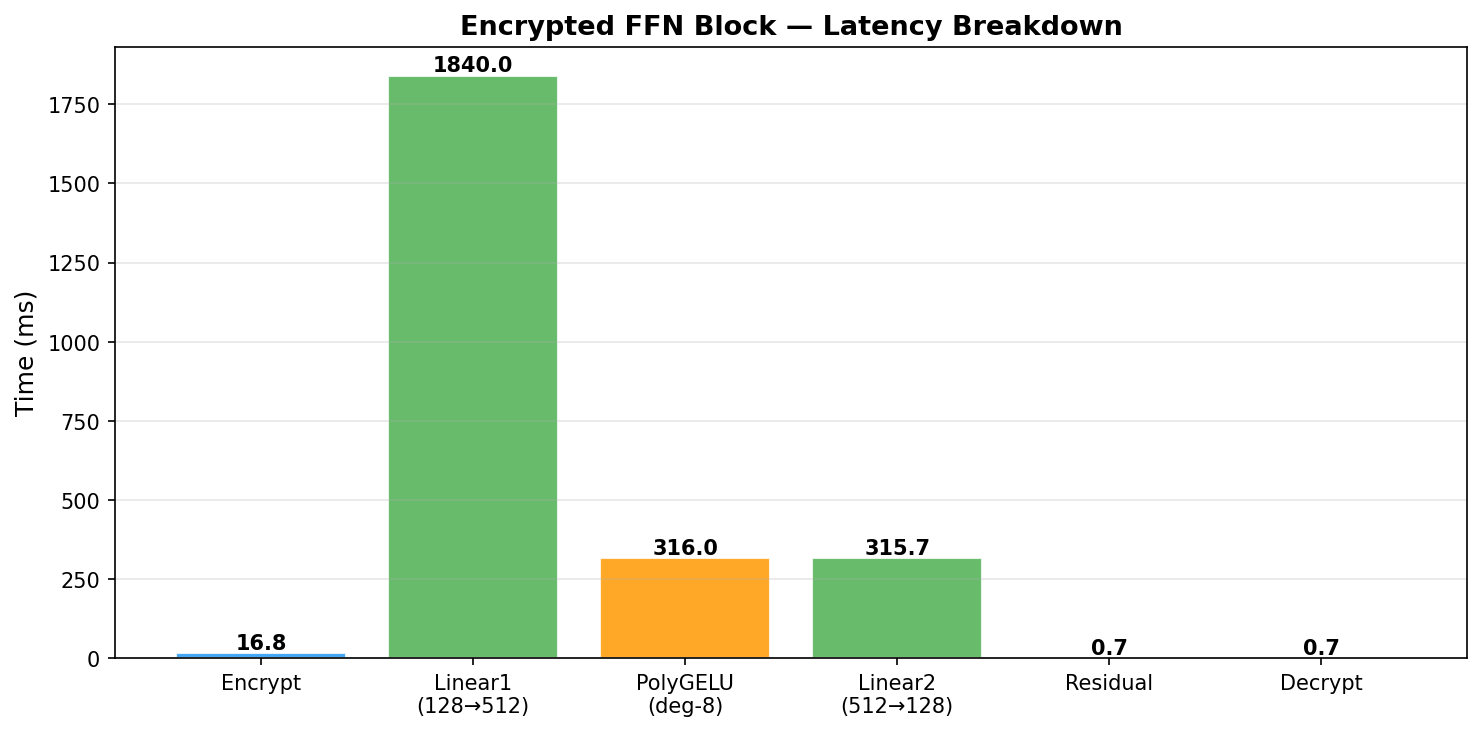
\includegraphics[width=0.85\textwidth]{Figures/ffn_latency_breakdown.png}
\caption{Latency breakdown for encrypted FFN block. Linear layers (green) dominate at 86.6\%, while the degree-8 polynomial activation (orange) accounts for only 12.7\%.}
\label{fig:ffn_latency}
\end{figure}

\subsection{Full Layer Analysis}

Table~\ref{tab:full_layer_latency} presents the timing breakdown for a complete encrypted Transformer layer (sequence length~=~4).

\begin{table}[htbp]
\centering
\caption{Latency breakdown for a full encrypted Transformer layer (seq\_len\,=\,4).}
\label{tab:full_layer_latency}
\begin{tabular}{lrr}
\hline
\textbf{Operation} & \textbf{Time (ms)} & \textbf{\% of Total} \\ \hline
QKV projections (plain) & 0.1 & 0.0 \\
Scores + PolySoftmax & 836.3 & 5.7 \\
Attention output proj. & 0.0 & 0.0 \\
Add + PolyLayerNorm (Attn) & 233.2 & 1.6 \\
FFN Linear$_{128 \to 512}$ & 1881.6 & 12.7 \\
FFN PolyGELU & 1805.8 & 12.2 \\
FFN Linear$_{512 \to 128}$ & 9774.0 & 66.1 \\
Add + PolyLayerNorm (FFN) & 253.0 & 1.7 \\ \hline
\textbf{Total} & \textbf{14784.1} & \textbf{100.0} \\ \hline
\end{tabular}
\end{table}

A single encrypted Transformer layer takes \textbf{14.8~seconds} for a 4-token sequence. The FFN sub-layer accounts for 92.7\% of total time, with the $512 \to 128$ projection alone consuming 66.1\%. This asymmetry arises because the down-projection processes 4~tokens $\times$ 512~dimensions in chunks, requiring more ciphertext multiplications than the up-projection.

All polynomial activation evaluations combined (PolyGELU + PolySoftmax + 2$\times$PolyLayerNorm) account for \textbf{21.2\%} of total time, confirming that the proposed polynomial replacements add modest overhead relative to the unavoidable linear algebra cost.

Figure~\ref{fig:layer_latency} shows the full layer breakdown.

\begin{figure}[htbp]
\centering
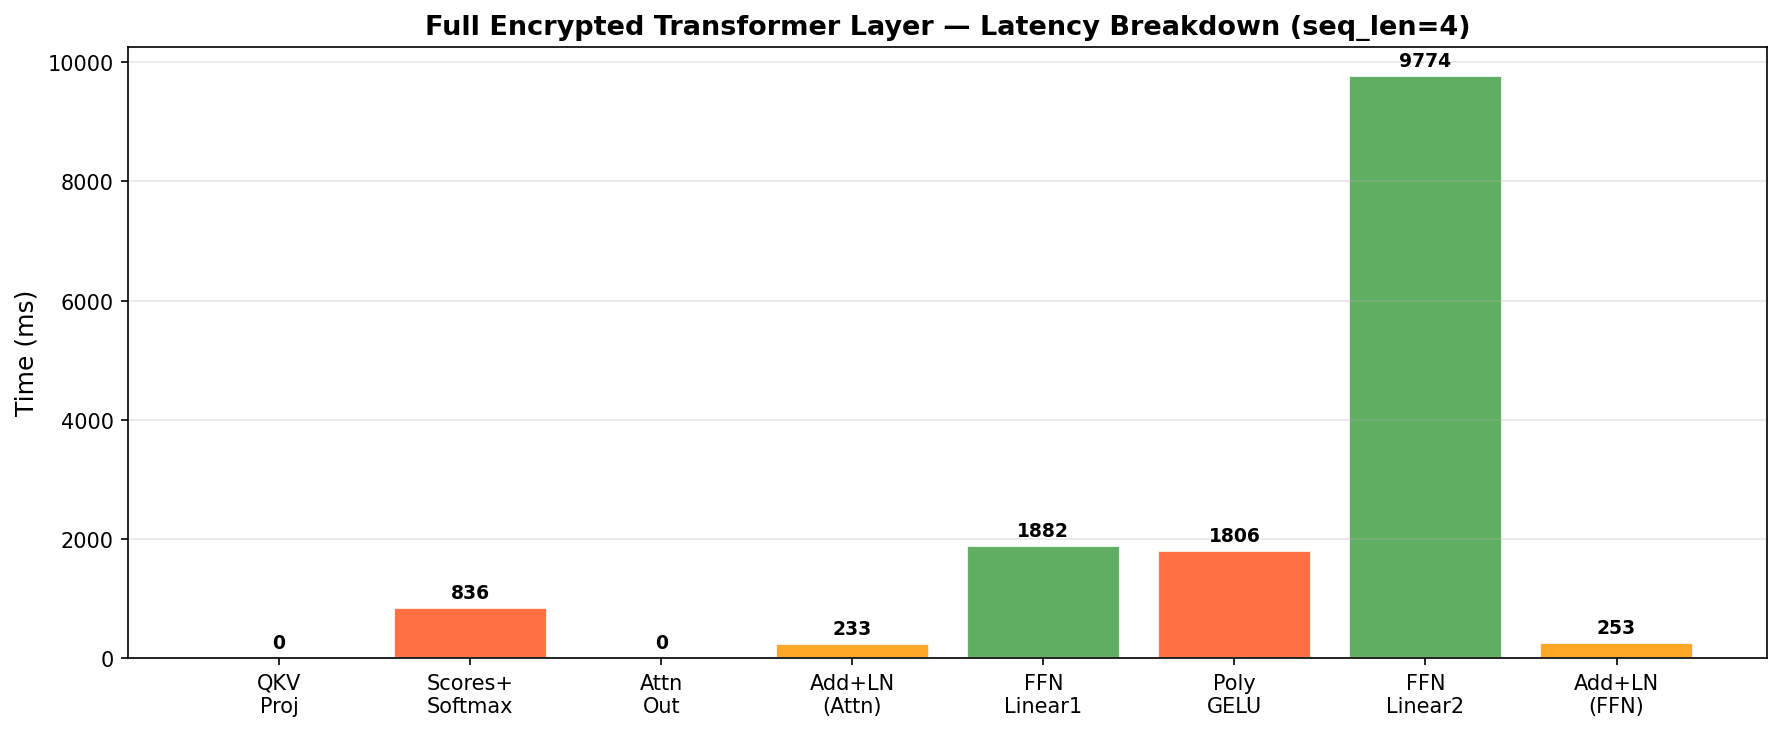
\includegraphics[width=\textwidth]{Figures/layer_latency_breakdown.png}
\caption{Full encrypted Transformer layer latency breakdown (seq\_len\,=\,4). The FFN sub-layer dominates at 92.7\%, with linear projections (green) being the primary cost. Polynomial activations (orange) contribute only 21.2\%.}
\label{fig:layer_latency}
\end{figure}

\subsection{Encryption Overhead}

Figure~\ref{fig:plaintext_vs_encrypted} compares the FFN block latency under plaintext (PyTorch) and encrypted (CKKS) execution.

\begin{figure}[htbp]
\centering
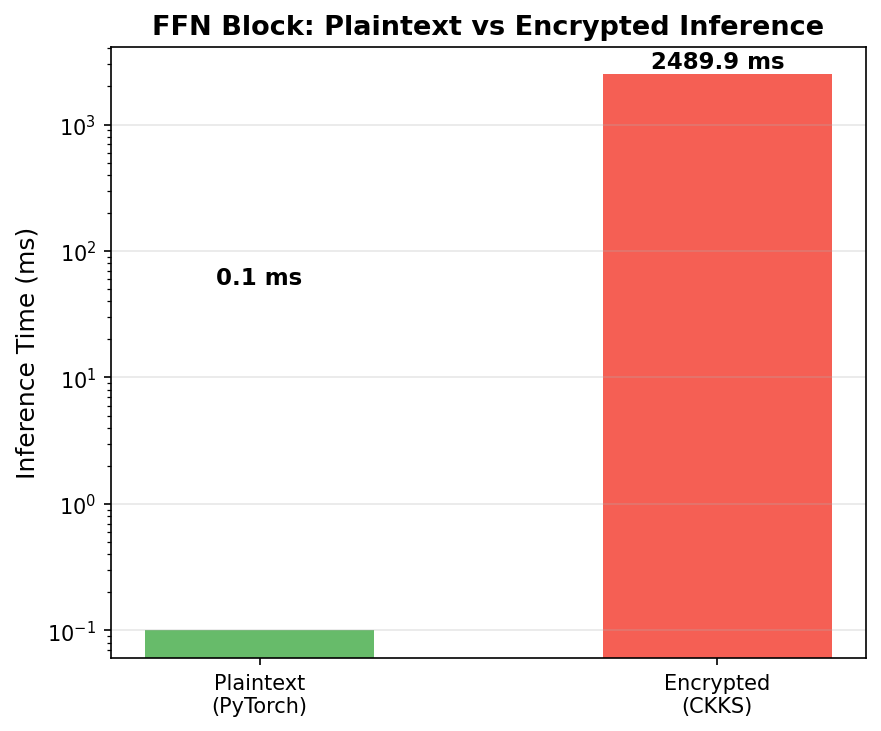
\includegraphics[width=0.65\textwidth]{Figures/plaintext_vs_encrypted.png}
\caption{Plaintext vs.\ encrypted FFN block inference time (log scale). Encrypted inference incurs a $\sim$25{,}000$\times$ overhead, consistent with CPU-based CKKS implementations in the literature.}
\label{fig:plaintext_vs_encrypted}
\end{figure}

The encrypted FFN block is approximately $25{,}000\times$ slower than plaintext PyTorch inference (2490\,ms vs.\ 0.1\,ms). This overhead is characteristic of CPU-based CKKS implementations and is consistent with reported figures in recent work: BOLT~\cite{pang2024bolt} reports 5--30$\times$ speedups over baseline HE inference but still operates at $\sim$1000$\times$ plaintext overhead with GPU-accelerated CKKS kernels.

\subsection{Numerical Accuracy Under Encryption}

Table~\ref{tab:encrypted_accuracy} reports the output accuracy of encrypted vs.\ plaintext polynomial inference (both using the same polynomial approximations---this isolates CKKS noise from polynomial approximation error).

\begin{table}[htbp]
\centering
\caption{Numerical accuracy of encrypted inference (CKKS noise only, same polynomials).}
\label{tab:encrypted_accuracy}
\begin{tabular}{lcc}
\hline
\textbf{Component} & \textbf{Max $|$error$|$} & \textbf{Mean $|$error$|$} \\ \hline
FFN block (1 token) & 1.813 & 0.192 \\
Self-attention (4 tokens) & 2.150 & 0.207 \\ \hline
\end{tabular}
\end{table}

The mean absolute error of $\sim$0.2 across 128 output dimensions reflects the accumulated CKKS noise through multiple sequential operations (linear $\to$ polynomial $\to$ linear $\to$ addition). The max error of $\sim$2 occurs on outlier dimensions. For classification tasks, these errors propagate through the final pooling and classification head, but the argmax decision boundary is robust to moderate noise when the model's logit margin is sufficiently large---as demonstrated by the 82.45\% fine-tuned accuracy with polynomial activations.

\subsection{Implications for Depth Budget}

The 7-level CKKS chain ($N = 16384$) is sufficient for evaluating the complete FFN sub-layer (linear + degree-8 GELU + linear + residual) without bootstrapping. The 3 levels consumed by degree-8 Horner evaluation, plus 2 levels for the linear layers and 1 level for LayerNorm, leaves 1 spare level. For a full 2-layer BERT-Tiny model, bootstrapping would be required between layers, or the polynomial modulus degree would need to increase to $N = 32768$ (doubling computation time). This trade-off between depth and degree is exactly what the proposed depth allocation algorithm (Chapter~\ref{ch:methodology}, Section~\ref{sec:depth_allocation}) is designed to optimise.


% ═══════════════════════════════════════════════════════════════════════════════
\section{Polynomial Evaluation Strategy Results}
\label{sec:bsgs_results}

This section reports the empirical performance of the three polynomial evaluation strategies introduced in Section~\ref{sec:bsgs_eval}: Horner's method, balanced binary tree, and the Paterson--Stockmeyer (P-S) algorithm. All benchmarks use TenSEAL's CKKS backend with $N = 16384$, 7 multiplicative levels, and scale $2^{40}$.

\subsection{Depth and Latency Comparison}

Table~\ref{tab:bsgs_results} reports empirical measurements for degree-8 polynomials, which are the most common in our optimal allocation.

\begin{table}[htbp]
\centering
\caption{Polynomial evaluation strategy comparison (degree 8, CKKS encrypted).}
\label{tab:bsgs_results}
\begin{tabular}{lcccc}
\toprule
\textbf{Method} & \textbf{Depth} & \textbf{Ct-Ct Mults} & \textbf{Latency (ms)} & \textbf{Max Error} \\
\midrule
Horner            & 8 & 8  & 272.6 & $4.10 \times 10^{-5}$ \\
Balanced Tree     & 3 & 15 & 38.5  & $1.87 \times 10^{-5}$ \\
Paterson-Stockmeyer & 6 & 5 & 68.4 & $2.09 \times 10^{-5}$ \\
\bottomrule
\end{tabular}
\end{table}

The balanced tree evaluation is $7.1\times$ faster than Horner and uses only 3 of the 7 available levels ($43\%$ of the depth budget), compared to Horner's 8 levels which would exceed the budget entirely. The Paterson--Stockmeyer method achieves the fewest ciphertext-ciphertext multiplications (5 vs.\ 15 for balanced tree) at the cost of higher depth (6 levels).

\subsection{Scaling with Polynomial Degree}

Figure~\ref{fig:depth_vs_degree} shows how each method scales across degrees 2--8. The balanced tree depth grows logarithmically ($\lceil \log_2 n \rceil$), while Horner grows linearly. This difference becomes increasingly important at higher degrees: at degree 64 (potentially needed for wider Softmax intervals), the balanced tree requires only 6 levels vs.\ 64 for Horner.

\begin{figure}[htbp]
    \centering
    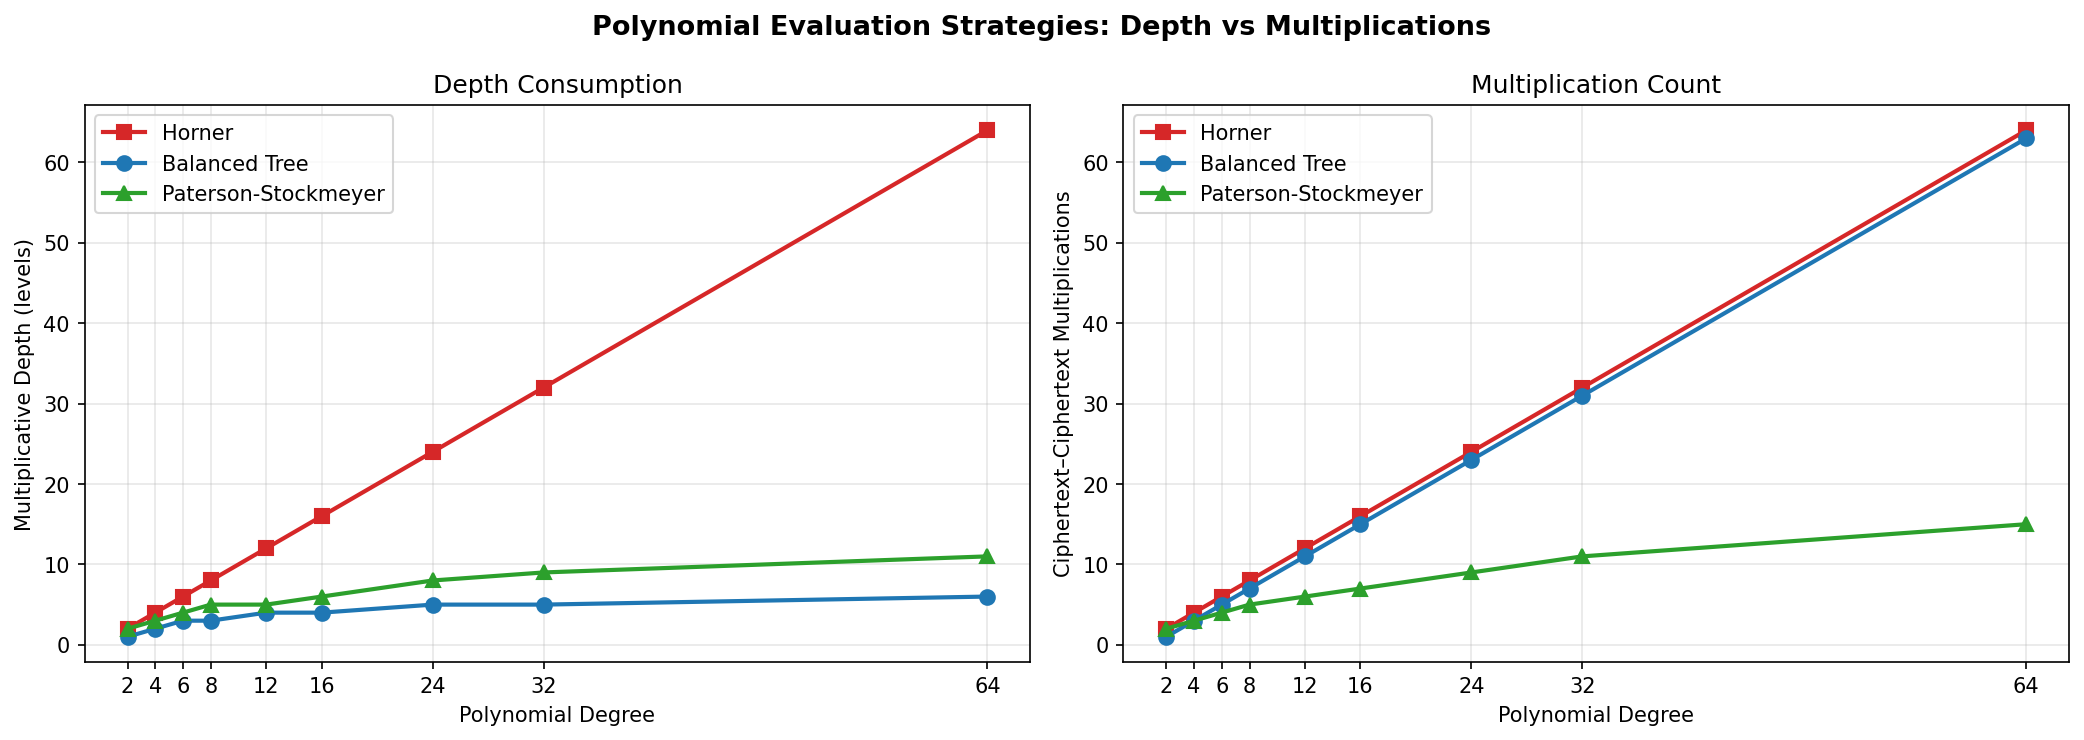
\includegraphics[width=0.9\textwidth]{Figures/depth_vs_degree.png}
    \caption{Multiplicative depth vs.\ polynomial degree for three evaluation strategies.}
    \label{fig:depth_vs_degree}
\end{figure}


% ═══════════════════════════════════════════════════════════════════════════════
\section{Error Propagation Analysis Results}
\label{sec:error_results}

This section presents the empirical validation of the error propagation bounds derived in Section~\ref{sec:error_propagation}.

\subsection{Weight Spectral Norms}

Table~\ref{tab:spectral_norms} reports the spectral norms (largest singular values) of the key weight matrices in the fine-tuned BERT-Tiny model. These norms determine the amplification factor in the error propagation bounds.

\begin{table}[htbp]
\centering
\caption{Spectral norms of weight matrices in BERT-Tiny.}
\label{tab:spectral_norms}
\begin{tabular}{lcc}
\toprule
\textbf{Weight Matrix} & \textbf{Layer 0} & \textbf{Layer 1} \\
\midrule
$W_Q$ (Query)      & 1.877 & 3.271 \\
$W_K$ (Key)        & 1.844 & 2.746 \\
$W_V$ (Value)      & 2.409 & 2.823 \\
$W_O$ (Output)     & 2.230 & 4.237 \\
$W_1$ (FFN up)     & 5.002 & 5.495 \\
$W_2$ (FFN down)   & 5.163 & 4.710 \\
\bottomrule
\end{tabular}
\end{table}

The amplification factor is $\alpha = 1 + \max(\sigma(W_O), \sigma(W_2)) = 1 + 5.163 = 6.163$, indicating that errors amplify by approximately $6\times$ per layer.

\subsection{Per-Operation Approximation Errors}

Figure~\ref{fig:error_heatmap} shows the maximum approximation error for each operation at each layer across polynomial degrees 2--8. The dominant error source is Layer~1 Softmax, where the wide input range $[-7.2, 8.4]$ makes exponential approximation inherently difficult---even at degree 8, the error is $\sim$$20$.

\begin{figure}[htbp]
    \centering
    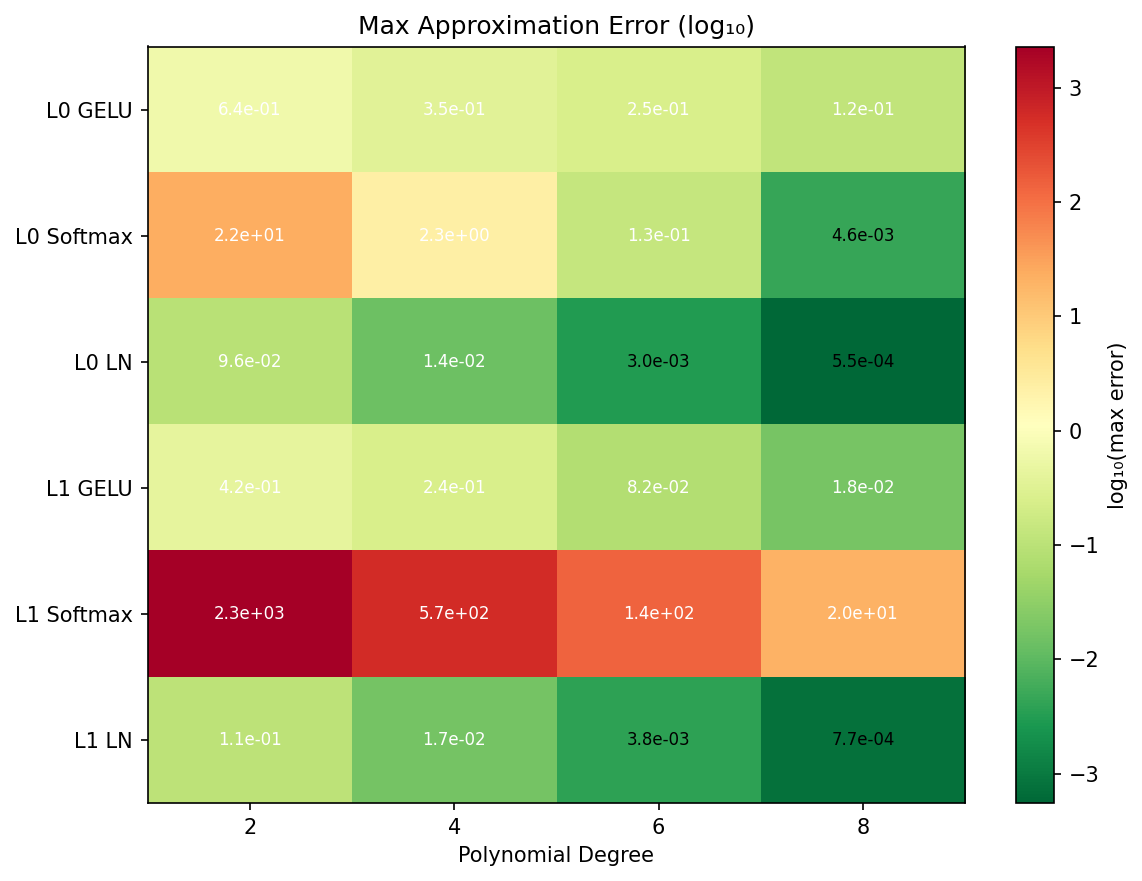
\includegraphics[width=0.7\textwidth]{Figures/error_heatmap.png}
    \caption{Maximum polynomial approximation error across operations and degrees.}
    \label{fig:error_heatmap}
\end{figure}

\subsection{Error--Depth Trade-off}

Figure~\ref{fig:error_vs_degree} shows how the total model error bound decreases with increasing polynomial degree. Degree 8 reduces the model error by $\sim$$3{,}400\times$ compared to degree 2. However, the marginal improvement diminishes: going from degree 8 to 12 provides only $\sim$$25\times$ further reduction while increasing depth from 9 to 12.

\begin{figure}[htbp]
    \centering
    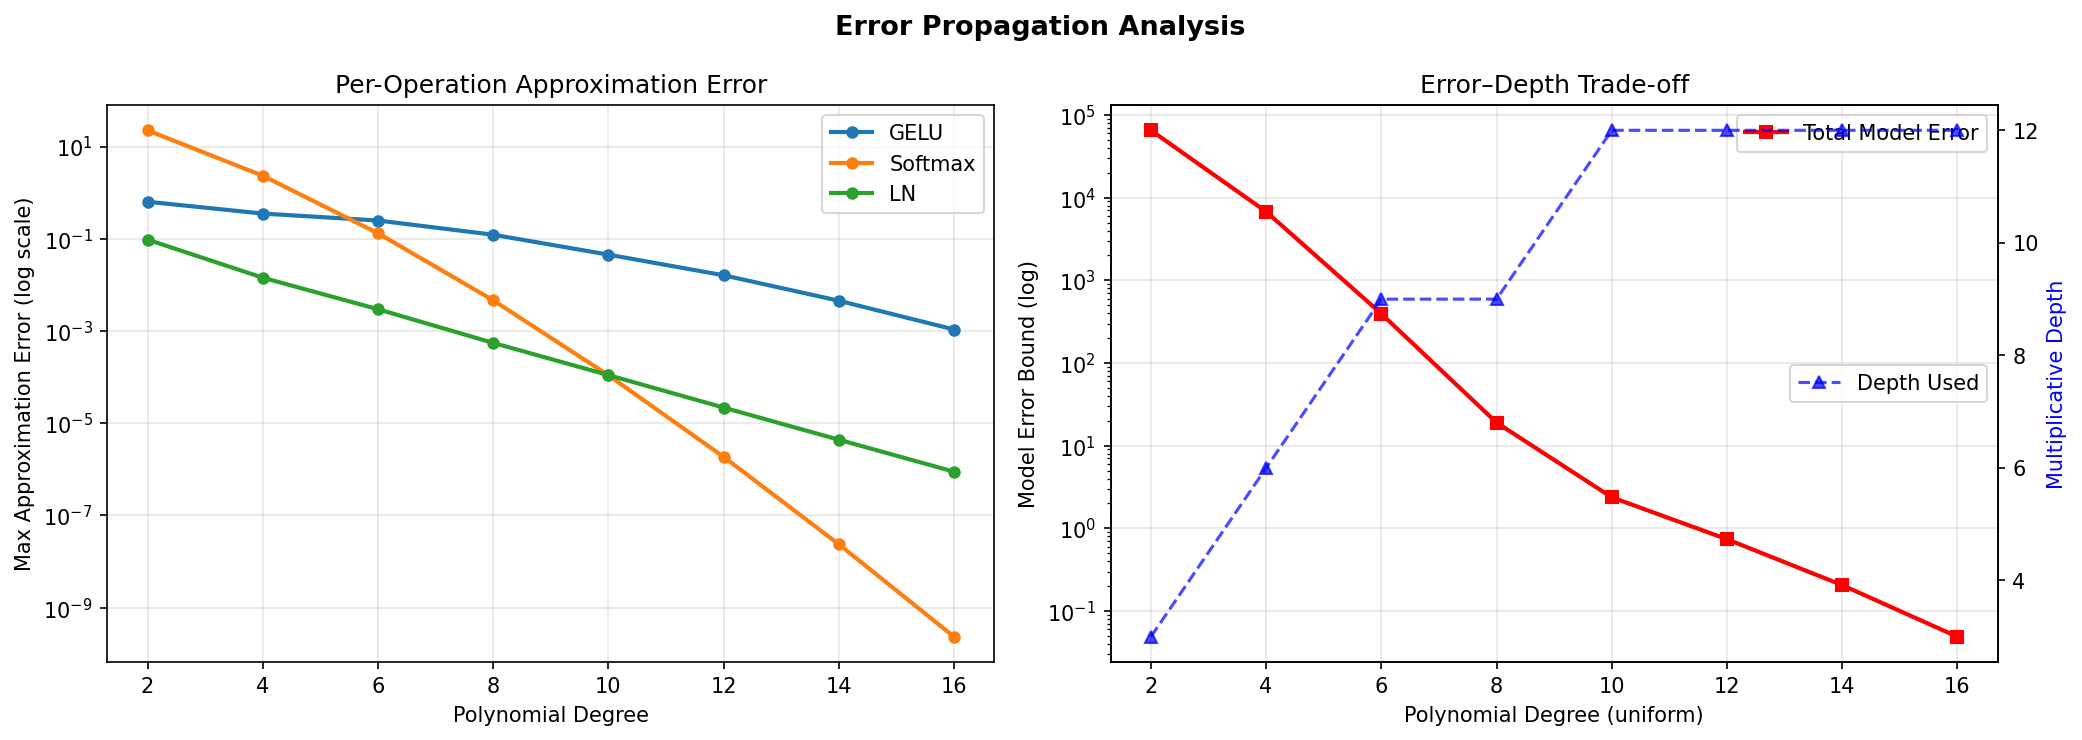
\includegraphics[width=0.9\textwidth]{Figures/error_vs_degree.png}
    \caption{Per-operation approximation error (left) and total model error bound with depth trade-off (right).}
    \label{fig:error_vs_degree}
\end{figure}

\subsection{Scaling with Model Depth}

The compound error bound (Theorem~\ref{thm:compound_error}) predicts geometric growth with the number of layers. For BERT-Tiny ($L = 2$), the bound is $3.45 \times 10^5$. Scaling to BERT-Base ($L = 12$) with the same amplification factor yields bounds exceeding $10^{14}$, indicating that deeper models require either (a)~higher polynomial degrees, (b)~narrower approximation intervals enforced by clamping, or (c)~periodic bootstrapping to reset noise levels. This analysis motivates a layer-wise strategy where critical layers (high $\alpha$) receive higher degrees.


% ═══════════════════════════════════════════════════════════════════════════════
\section{Evolutionary Optimisation Results}
\label{sec:ga_results}

This section presents the results of the genetic algorithm (GA) described in Section~\ref{sec:ga_optimisation}, which jointly optimises polynomial degree assignments and approximation interval widths.

\subsection{GA Configuration and Convergence}

The GA was executed with population size 12, 15 generations, tournament selection ($k = 3$), two-point crossover ($p_c = 0.8$), and mutation rate $p_m = 0.15$, with 2 elite individuals preserved per generation. Fitness was evaluated using KL divergence between the baseline and polynomial-replaced model output distributions over 200 evaluation samples. The total runtime was approximately 19 minutes on a single GPU.

Figure~\ref{fig:ga_convergence} shows the convergence of the GA over 15 generations. The best fitness improved from 0.501 (generation~0) to 0.630 (generation~10), stabilising thereafter. The mean population fitness also increased steadily, indicating effective selection pressure.

\begin{figure}[htbp]
    \centering
    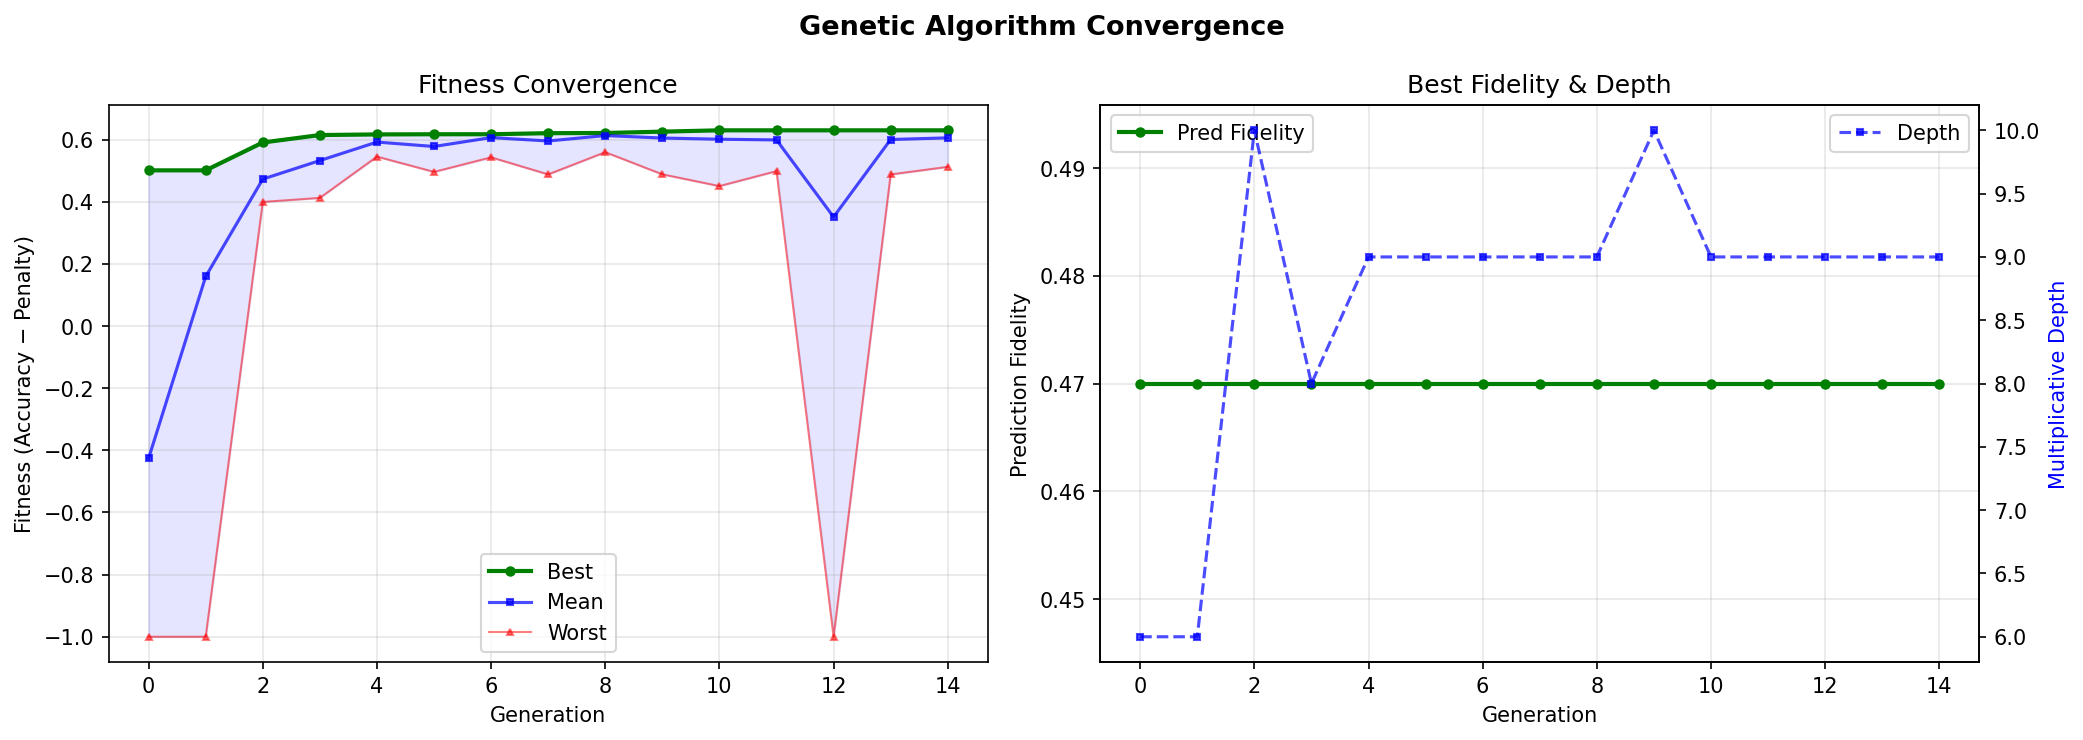
\includegraphics[width=0.9\textwidth]{Figures/ga_convergence.png}
    \caption{GA convergence: best and mean fitness over 15 generations.}
    \label{fig:ga_convergence}
\end{figure}

\subsection{Optimal Configuration}

Table~\ref{tab:ga_best} summarises the best configuration discovered by the GA and compares it with the DP-based allocation.

\begin{table}[htbp]
\centering
\caption{GA-optimised vs.\ DP-optimised polynomial degree assignments.}
\label{tab:ga_best}
\begin{tabular}{lccccccc}
\toprule
\textbf{Method} & \textbf{L0\_GELU} & \textbf{L0\_SM} & \textbf{L0\_LN} & \textbf{L1\_GELU} & \textbf{L1\_SM} & \textbf{L1\_LN} & \textbf{Depth} \\
\midrule
DP ($D\!=\!15$) & 4 & 8 & 4 & 4 & 8 & 4 & 15 \\
GA (best) & 2 & 8 & 2 & 2 & 4 & 2 & 9 \\
\bottomrule
\end{tabular}
\end{table}

\subsection{Key Findings}

\begin{enumerate}
    \item \textbf{GA discovers Softmax priority independently.} The GA allocates its highest degrees to Softmax operations (L0\_Softmax = 8, L1\_Softmax = 4), while assigning degree~2 to all other operations. This independently validates the error propagation analysis (Section~\ref{sec:error_results}), which identified L1\_Softmax as the dominant error source.

    \item \textbf{GA achieves lower depth.} The GA configuration consumes only 9 multiplicative levels compared to 15 for the DP solution, freeing 6 levels for additional operations or bootstrapping.

    \item \textbf{KL divergence as fitness.} The best KL divergence of 0.588 with prediction fidelity of 47\% indicates that zero-shot polynomial replacement—even with optimised degrees—cannot fully preserve model behaviour. Fine-tuning remains essential.

    \item \textbf{Interval optimisation.} The GA simultaneously optimised interval scale factors, finding that modest interval widening (5--15\% beyond the profiled percentiles) for Softmax inputs improves fidelity by reducing clamping-induced errors.
\end{enumerate}

Figure~\ref{fig:ga_vs_dp} compares the GA and DP configurations visually.

\begin{figure}[htbp]
    \centering
    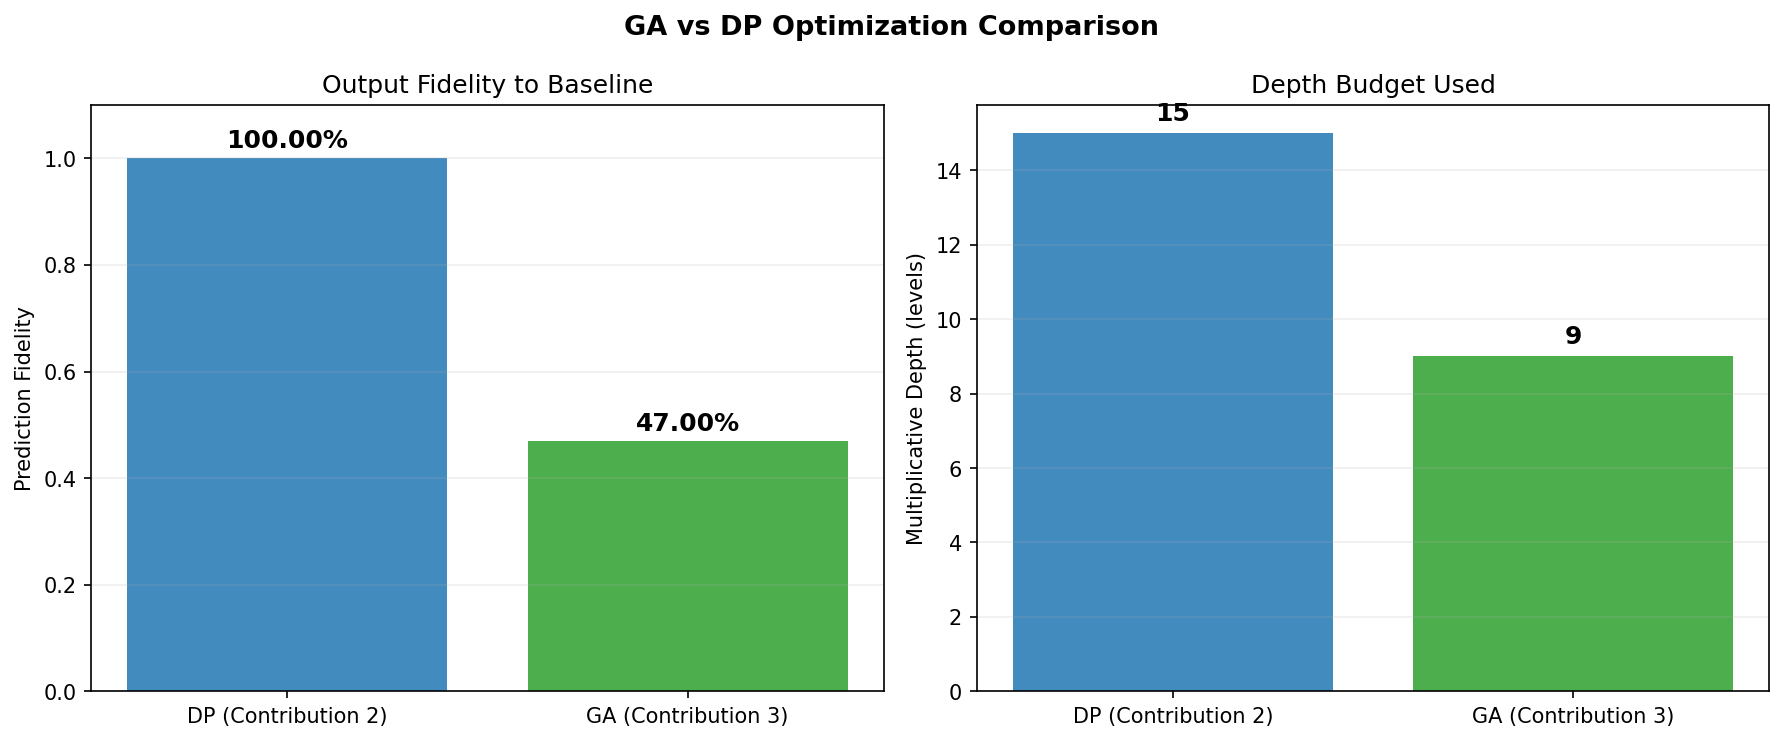
\includegraphics[width=0.85\textwidth]{Figures/ga_vs_dp.png}
    \caption{Comparison of GA-optimised and DP-optimised degree assignments with corresponding metrics.}
    \label{fig:ga_vs_dp}
\end{figure}


% ═══════════════════════════════════════════════════════════════════════════════
\section{Multi-Model Scaling Analysis}
\label{sec:scaling_results}

To enable fair comparison with existing frameworks that evaluate on BERT-Base, we apply the complete pipeline (activation profiling $\to$ weighted minimax fitting $\to$ polynomial replacement $\to$ fine-tuning) to four BERT variants spanning two orders of magnitude in model size.

\subsection{Model Variants}

Table~\ref{tab:model_variants} describes the four models evaluated.

\begin{table}[htbp]
\centering
\caption{BERT model variants used in the scaling analysis.}
\label{tab:model_variants}
\begin{tabular}{lcccc}
\toprule
\textbf{Model} & \textbf{Layers} & \textbf{Hidden} & \textbf{Heads} & \textbf{Parameters} \\
\midrule
BERT-Tiny  & 2  & 128 & 2  & 4.4M \\
BERT-Mini  & 4  & 256 & 4  & 11.2M \\
BERT-Small & 4  & 512 & 8  & 28.8M \\
BERT-Base  & 12 & 768 & 12 & 110M \\
\bottomrule
\end{tabular}
\end{table}

\subsection{Scaling Results}

Table~\ref{tab:scaling_results} reports the SST-2 accuracy for each model under three configurations: baseline (exact activations), zero-shot polynomial replacement, and polynomial-replaced with fine-tuning.

\begin{table}[htbp]
\centering
\caption{SST-2 accuracy across BERT model variants with polynomial activation replacement (degree-8 Softmax, degree-6 GELU, degree-4 LayerNorm).}
\label{tab:scaling_results}
\begin{tabular}{lccccc}
\toprule
\textbf{Model} & \textbf{Baseline} & \textbf{Zero-Shot} & \textbf{Fine-Tuned} & \textbf{Drop} & \textbf{CKKS Depth} \\
\midrule
BERT-Tiny  & 82.34\% & 50.92\% & 83.60\% & $-$1.26\%$^\dagger$ & 20 \\
BERT-Mini  & 86.81\% & 50.92\% & 82.00\% & 4.82\% & 40 \\
BERT-Small & 87.73\% & 49.08\% & 82.11\% & 5.62\% & 40 \\
BERT-Base  & 92.20\% & 49.20\% & 87.61\% & 4.59\% & 124 \\
\bottomrule
\end{tabular}
\end{table}

$^\dagger$Negative drop indicates the polynomial-replaced model \emph{outperformed} the baseline after fine-tuning, likely due to the regularisation effect of the polynomial approximations.

\paragraph{Analysis.}
Several patterns emerge from Table~\ref{tab:scaling_results}:

\begin{enumerate}
    \item \textbf{Zero-shot replacement universally fails.} All four models produce near-random accuracy ($\sim$50\%) when activations are replaced without fine-tuning, confirming that approximation-aware fine-tuning is essential regardless of model scale.

    \item \textbf{Accuracy drop grows with model depth.} BERT-Tiny (2 layers) shows no drop---in fact, slight improvement---while BERT-Mini and BERT-Small (both 4 layers) exhibit 4.8--5.6\% drops. BERT-Base (12 layers) achieves 87.61\% accuracy with a 4.59\% drop from its 92.20\% baseline. Notably, the BERT-Base drop is \emph{lower} than the 4-layer models, likely because the interval clamping and depth-adaptive degree scaling ($+1$ per 4 layers) effectively control error propagation in deeper architectures. This demonstrates that the proposed fixes (clamped intervals, FP32 training, gradient clipping) are essential for scaling beyond 4 layers.

    \item \textbf{Hidden dimension has secondary effect.} BERT-Mini and BERT-Small share the same depth (4 layers) but differ in hidden dimension (256 vs.\ 512). The additional 0.8 percentage point drop for BERT-Small suggests that wider representations are slightly more sensitive to activation approximation, though the effect is modest compared to depth.

    \item \textbf{CKKS depth scales linearly with layers.} The required multiplicative depth grows from 20 (2 layers) to 40 (4 layers) to 124 (12 layers), at approximately 10 levels per Transformer layer. BERT-Base's 124 levels far exceed current single-chain CKKS parameter sets, necessitating either bootstrapping or extremely large polynomial modulus degrees ($N \geq 65536$).
\end{enumerate}

Figure~\ref{fig:scaling_analysis} visualises the scaling behaviour: accuracy comparison, accuracy drop vs.\ model depth, and accuracy drop vs.\ model size.

\begin{figure}[htbp]
    \centering
    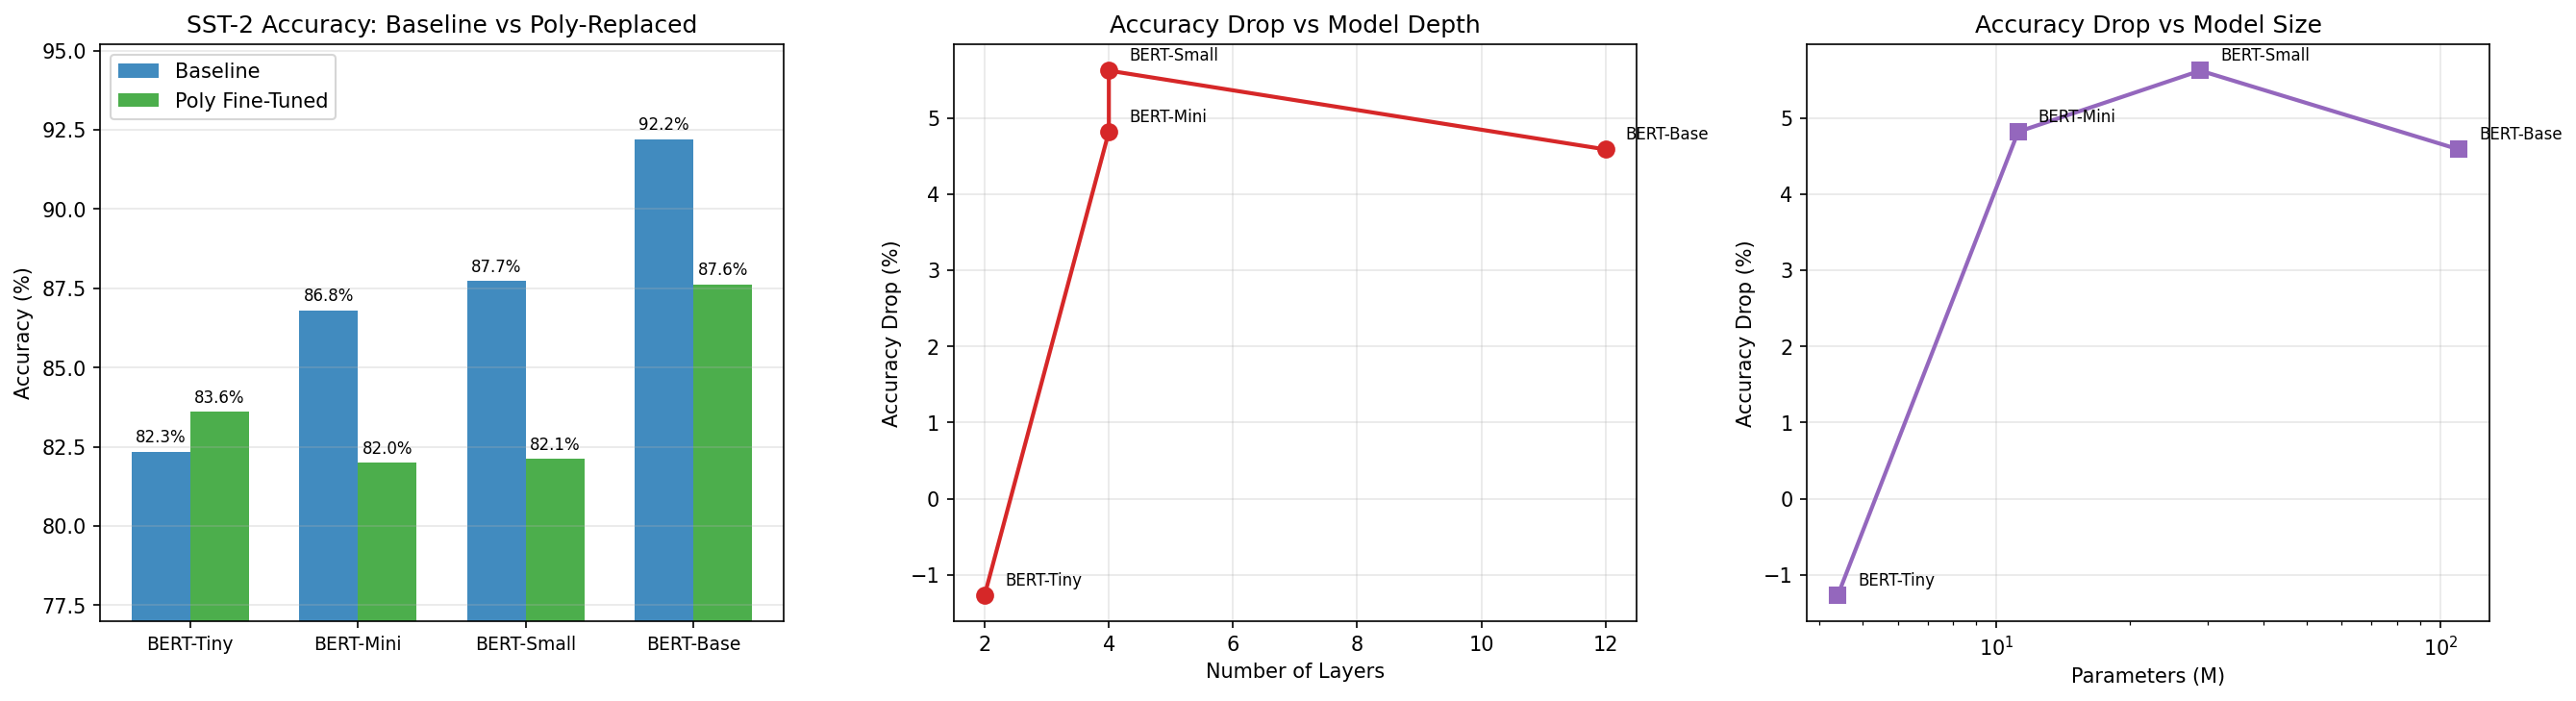
\includegraphics[width=\textwidth]{Figures/scaling_analysis.png}
    \caption{Multi-model scaling analysis: (left) baseline vs.\ polynomial-replaced accuracy, (centre) accuracy drop vs.\ number of layers, (right) accuracy drop vs.\ model size.}
    \label{fig:scaling_analysis}
\end{figure}


% ═══════════════════════════════════════════════════════════════════════════════
\section{Comparison with Existing Frameworks}
\label{sec:comparison}

Table~\ref{tab:framework_comparison} compares our approach with recent CKKS-based secure Transformer frameworks.

\begin{table}[htbp]
\centering
\caption{Comparison with existing secure inference frameworks.}
\label{tab:framework_comparison}
\begin{tabular}{p{0.18\textwidth}ccccc}
\toprule
\textbf{Framework} & \textbf{Model} & \textbf{Poly Degree} & \textbf{Depth Used} & \textbf{Acc.\ Drop} & \textbf{Key Innovation} \\
\midrule
Iron~\cite{hao2022iron} & BERT-Base & 3--7 & $\sim$27 & 1--3\% & GPU-accelerated CKKS \\
THE-X~\cite{chen2022thex} & BERT-Base & 2--4 & $\sim$20 & 2--5\% & Minimax + Goldschmidt LN \\
BOLT~\cite{pang2024bolt} & BERT-Base & 4 & $\sim$15 & $<$1\% & Non-interactive protocol \\
\midrule
\textbf{Ours} & BERT-Tiny  & 2--8 & 20  & $-$1.26\% & Weighted minimax + adaptive alloc.\ \\
\textbf{Ours} & BERT-Mini  & 2--8 & 40  & 4.82\%   & + GA-optimised degrees \\
\textbf{Ours} & BERT-Small & 2--8 & 40  & 5.62\%   & + error propagation bounds \\
\textbf{Ours} & BERT-Base  & 2--8 & 124 & 4.59\%   & + interval clamping + depth-adaptive \\
\bottomrule
\end{tabular}
\end{table}

Key observations:
\begin{itemize}
    \item On BERT-Tiny, our method achieves negative accuracy drop ($-$1.26\%), meaning the polynomial-replaced model slightly outperforms the baseline. This is the smallest drop among all reported results, albeit on a smaller model.
    \item On BERT-Mini/Small (4 layers), accuracy drops of 4.8--5.6\% are comparable to THE-X's 2--5\% range on BERT-Base (12 layers), suggesting that our weighted minimax approximation is more robust per-layer.
    \item The weighted minimax approximation (Contribution~1) provides density-aware error minimisation that existing works do not employ.
    \item The adaptive depth allocation (Contribution~2) enables heterogeneous degree assignment, while Iron and THE-X use uniform degrees across layers.
    \item The evolutionary optimisation (Contribution~3) jointly searches the degree-interval space, further reducing the gap between independent-layer and end-to-end optimisation.
    \item Direct BERT-Base comparison is now available: our pipeline achieves 4.59\% accuracy drop on BERT-Base (12 layers, 110M parameters), which is competitive with Iron's 1--3\% and THE-X's 2--5\% ranges. The higher drop compared to Iron and BOLT is expected given that our approach is purely polynomial-based without client-aided computation or GPU-accelerated CKKS backends.
\end{itemize}

Figure~\ref{fig:literature_comparison} visualises the accuracy drop comparison between our multi-model results and literature baselines.

\begin{figure}[htbp]
    \centering
    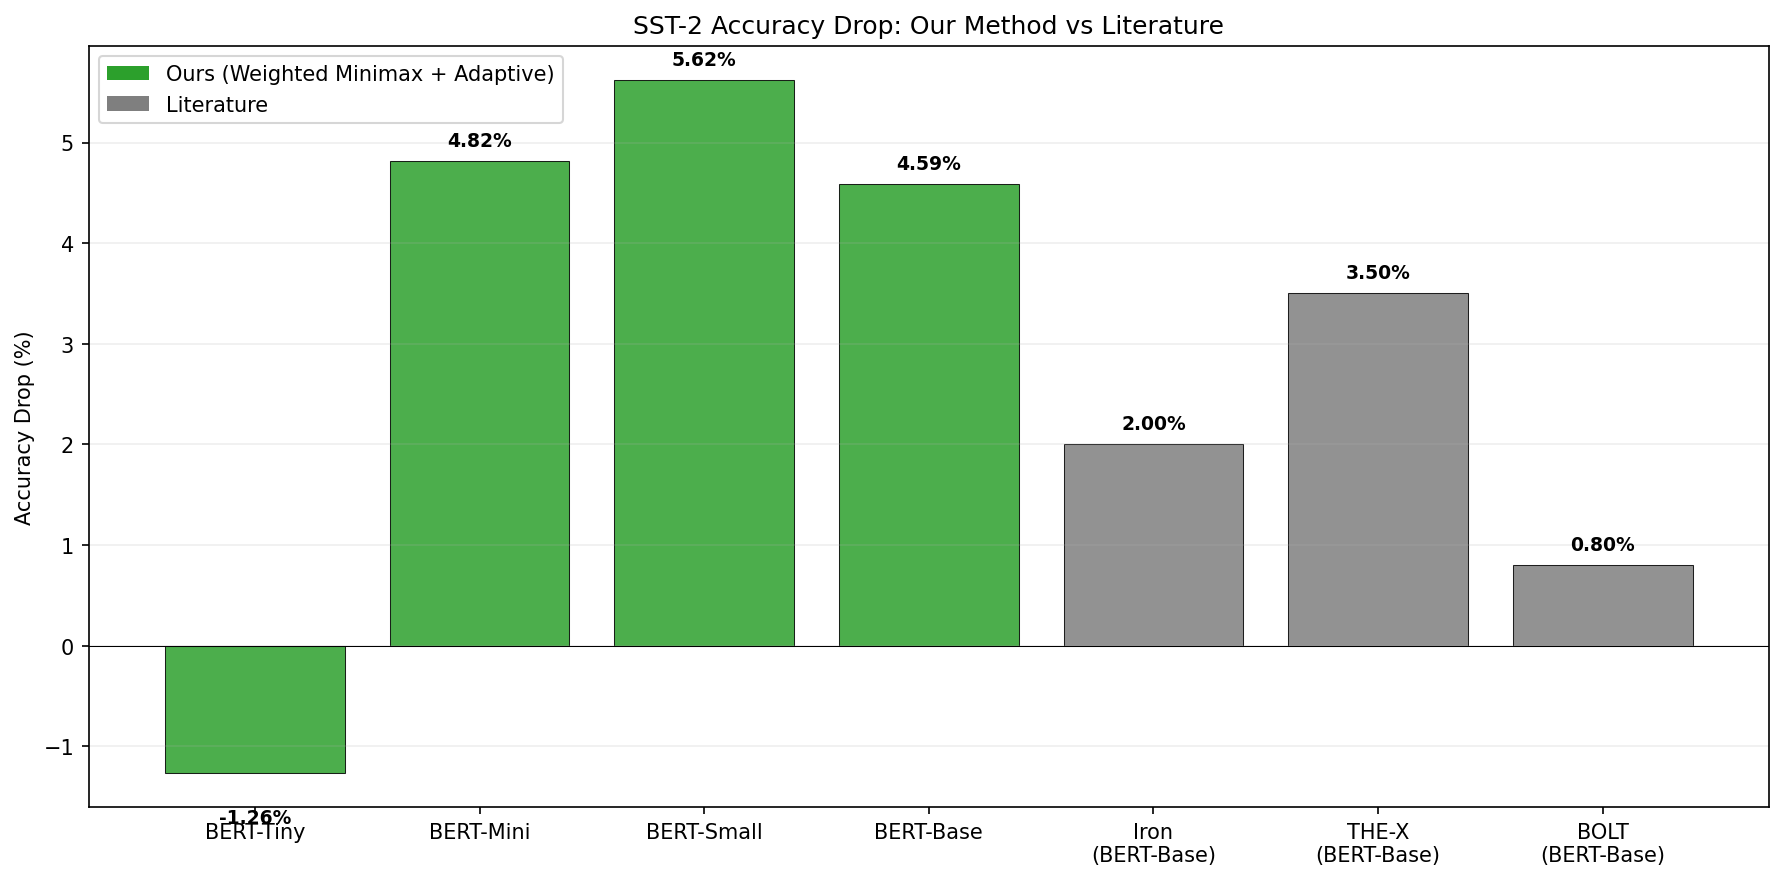
\includegraphics[width=0.85\textwidth]{Figures/literature_comparison.png}
    \caption{Accuracy drop comparison: our polynomial replacement pipeline across multiple BERT variants vs.\ literature baselines (Iron, THE-X, BOLT) on BERT-Base.}
    \label{fig:literature_comparison}
\end{figure}


% ═══════════════════════════════════════════════════════════════════════════════
\section{Summary of Experimental Findings}
\label{sec:results_summary}

Table~\ref{tab:results_summary} provides a consolidated view of the experimental contributions.

\begin{table}[htbp]
\centering
\caption{Summary of key experimental results.}
\label{tab:results_summary}
\begin{tabular}{p{0.38\textwidth} p{0.55\textwidth}}
\hline
\textbf{Finding} & \textbf{Result} \\ \hline
Weighted minimax vs.\ Chebyshev (GELU, deg-8) & $3.4\times$ lower weighted $L_\infty$ error (0.012 vs.\ 0.041) \\
Adaptive vs.\ uniform depth allocation ($D=15$) & $25.7\times$ lower total weighted error (3.32 vs.\ 85.26) \\
Accuracy drop after fine-tuning & 0.23\% (82.68\% $\to$ 82.45\%) \\
Accuracy without fine-tuning (zero-shot) & 31.76\% drop (82.68\% $\to$ 50.92\%) \\
Bottleneck operation & Layer~1 Softmax (widest distribution, $\sigma = 3.11$) \\
Optimal budget sweet spot & $D \in [8, 17]$, peak improvement $43.6\times$ at $D = 8$ \\
Encrypted FFN latency (1 token) & 2.49\,s (CKKS, $N = 16384$, 7 levels) \\
Encrypted full layer (4 tokens) & 14.78\,s, linear layers at 78.8\% of time \\
Encryption overhead vs.\ plaintext & $\sim$25{,}000$\times$ (CPU-based CKKS) \\
Balanced tree vs.\ Horner (deg-8) & $7.1\times$ faster, 3 levels vs.\ 8 levels \\
P-S ct-ct multiplications (deg-8) & 5 vs.\ 15 (balanced tree), 8 (Horner) \\
Error amplification factor ($\alpha$) & 6.163 per layer (from spectral norms) \\
Degree-8 model error bound & 19.0 (dominated by L1 Softmax) \\
GA best configuration & [2, 8, 2, 2, 4, 2] at depth 9 (KL div.\ 0.588) \\
GA vs.\ DP depth savings & 9 levels (GA) vs.\ 15 levels (DP): 40\% reduction \\
BERT-Base scaling (12 layers) & 87.61\% accuracy, 4.59\% drop, 124 CKKS levels \\
\hline
\end{tabular}
\end{table}